% --- ANNAHME: Alle Pakete und Box-Definitionen aus dem Hauptdokument sind hier gültig ---
% --- Dieser Code-Block ist als Ersatz für das bestehende Kapitel 4 gedacht ---

\section{Quadratische Funktionen – Die Welt der Parabeln}
\label{sec:quadratische-funktionen_ueberarbeitet}

\begin{aufgabenumgebung}{Parameter-Check}
Betrachte die folgenden quadratischen Funktionen. Gib für jede Funktion die Werte der Koeffizienten $a, b$ und $c$ an. Was kannst du sofort über die Öffnungsrichtung, die Form (schmaler/breiter als Normalparabel) und den y-Achsenabschnitt sagen?
\begin{enumerate}
    \item $f(x) = 2x^2 - 4x + 5$
    \item $g(x) = -x^2 + 3x - 1$
    \item $h(x) = 0.25x^2 + 2$ (Achtung, welcher Koeffizient ist hier Null?)
    \item $k(x) = -3x^2 - 6x$ (Und hier?)
\end{enumerate}
\end{aufgabenumgebung}


\begin{loesungsumgebung}[loes:parameter-check-quadratisch]{Parameter-Check}
Die allgemeine Form einer quadratischen Funktion ist $f(x) = ax^2 + bx + c$. Die Koeffizienten $a, b$ und $c$ geben Aufschluss über verschiedene Eigenschaften der Parabel.

\begin{enumerate}[label=(\alph*)]
    \item \textbf{Funktion $f(x) = 2x^2 - 4x + 5$}
    \begin{itemize}
        \item Koeffizienten: $a = 2$, $b = -4$, $c = 5$.
        \item \textbf{Öffnungsrichtung:} Da $a = 2 > 0$ ist, ist die Parabel \textbf{nach oben geöffnet}.
        \item \textbf{Form:} Da $|a| = |2| = 2 > 1$ ist, ist die Parabel \textbf{schmaler} als die Normalparabel (sie ist gestreckt).
        \item \textbf{y-Achsenabschnitt:} Der Koeffizient $c = 5$ gibt den y-Achsenabschnitt an. Die Parabel schneidet die y-Achse im Punkt $(0|5)$.
    \end{itemize}

    \item \textbf{Funktion $g(x) = -x^2 + 3x - 1$}
    \begin{itemize}
        \item Koeffizienten: $a = -1$, $b = 3$, $c = -1$.
        \item \textbf{Öffnungsrichtung:} Da $a = -1 < 0$ ist, ist die Parabel \textbf{nach unten geöffnet}.
        \item \textbf{Form:} Da $|a| = |-1| = 1$ ist, hat die Parabel die \textbf{gleiche Form wie die Normalparabel} (ist weder schmaler noch breiter, nur nach unten geöffnet).
        \item \textbf{y-Achsenabschnitt:} Der Koeffizient $c = -1$ gibt den y-Achsenabschnitt an. Die Parabel schneidet die y-Achse im Punkt $(0|-1)$.
    \end{itemize}

    \item \textbf{Funktion $h(x) = 0.25x^2 + 2$}
    Um die Koeffizienten klar zu sehen, kann man die Funktion als $h(x) = 0.25x^2 + 0x + 2$ schreiben.
    \begin{itemize}
        \item Koeffizienten: $a = 0.25$, $b = 0$, $c = 2$.
        \item \textbf{Öffnungsrichtung:} Da $a = 0.25 > 0$ ist, ist die Parabel \textbf{nach oben geöffnet}.
        \item \textbf{Form:} Da $|a| = |0.25| = 0.25 < 1$ ist, ist die Parabel \textbf{breiter} als die Normalparabel (sie ist gestaucht).
        \item \textbf{y-Achsenabschnitt:} Der Koeffizient $c = 2$ gibt den y-Achsenabschnitt an. Die Parabel schneidet die y-Achse im Punkt $(0|2)$.
        \item \textit{Anmerkung (Achtung, welcher Koeffizient ist hier Null?):} Der Koeffizient $b$ ist hier Null ($b=0$). Dies bedeutet, dass die Parabel achsensymmetrisch zur y-Achse ist und ihr Scheitelpunkt auf der y-Achse bei $(0|c)$ liegt, also bei $(0|2)$.
    \end{itemize}

    \item \textbf{Funktion $k(x) = -3x^2 - 6x$}
    Um die Koeffizienten klar zu sehen, kann man die Funktion als $k(x) = -3x^2 - 6x + 0$ schreiben.
    \begin{itemize}
        \item Koeffizienten: $a = -3$, $b = -6$, $c = 0$.
        \item \textbf{Öffnungsrichtung:} Da $a = -3 < 0$ ist, ist die Parabel \textbf{nach unten geöffnet}.
        \item \textbf{Form:} Da $|a| = |-3| = 3 > 1$ ist, ist die Parabel \textbf{schmaler} als die Normalparabel (sie ist gestreckt).
        \item \textbf{y-Achsenabschnitt:} Der Koeffizient $c = 0$ gibt den y-Achsenabschnitt an. Die Parabel schneidet die y-Achse im Punkt $(0|0)$, d.h., sie verläuft durch den Ursprung des Koordinatensystems.
        \item \textit{Anmerkung (Und hier?):} Der Koeffizient $c$ ist hier Null ($c=0$). Dies bedeutet, dass die Parabel durch den Ursprung geht.
    \end{itemize}
\end{enumerate}

\end{loesungsumgebung}


\begin{aufgabenumgebung}{Parabeln skizzieren mit Wertetabelle}
\begin{enumerate}
    \item Erstelle eine Wertetabelle für die Normalparabel $f(x)=x^2$ für $x$-Werte von $-3$ bis $3$ (in Einerschritten). Zeichne den Graphen.
    \item Erstelle eine Wertetabelle für $g(x)=2x^2$ für dieselben x-Werte. Zeichne den Graphen in dasselbe Koordinatensystem wie $f(x)$. Was beobachtest du im Vergleich zur Normalparabel?
    \item Erstelle eine Wertetabelle für $h(x)=-0.5x^2+1$ für dieselben x-Werte. Zeichne den Graphen ebenfalls in dasselbe Koordinatensystem. Was beobachtest du?
\end{enumerate}
\end{aufgabenumgebung}


\begin{loesungsumgebung}[loes:parabeln-skizzieren-wertetabelle]{Parabeln skizzieren mit Wertetabelle}

\begin{enumerate}[label=(\alph*)]
    \item \textbf{Normalparabel $f(x)=x^2$} \\
    Wir erstellen eine Wertetabelle für $f(x)=x^2$ für die $x$-Werte von $-3$ bis $3$:
    \begin{itemize}
        \item $f(-3) = (-3)^2 = 9$
        \item $f(-2) = (-2)^2 = 4$
        \item $f(-1) = (-1)^2 = 1$
        \item $f(0) = (0)^2 = 0$
        \item $f(1) = (1)^2 = 1$
        \item $f(2) = (2)^2 = 4$
        \item $f(3) = (3)^2 = 9$
    \end{itemize}
    \textbf{Wertetabelle für $f(x)=x^2$:}
    \begin{center}
    \begin{tabular}{r r}
    \toprule
    \multicolumn{1}{c}{$x$} & \multicolumn{1}{c}{$f(x)=x^2$} \\
    \midrule
    $-3$ & $9$ \\
    $-2$ & $4$ \\
    $-1$ & $1$ \\
    $0$ & $0$ \\
    $1$ & $1$ \\
    $2$ & $4$ \\
    $3$ & $9$ \\
    \bottomrule
    \end{tabular}
    \end{center}
    Der Graph dieser Funktion ist die Normalparabel mit dem Scheitelpunkt im Ursprung $(0|0)$ und nach oben geöffnet.

    \item \textbf{Funktion $g(x)=2x^2$} \\
    Wir erstellen eine Wertetabelle für $g(x)=2x^2$ für dieselben $x$-Werte:
    \begin{itemize}
        \item $g(-3) = 2(-3)^2 = 2 \cdot 9 = 18$
        \item $g(-2) = 2(-2)^2 = 2 \cdot 4 = 8$
        \item $g(-1) = 2(-1)^2 = 2 \cdot 1 = 2$
        \item $g(0) = 2(0)^2 = 0$
        \item $g(1) = 2(1)^2 = 2$
        \item $g(2) = 2(2)^2 = 8$
        \item $g(3) = 2(3)^2 = 18$
    \end{itemize}
    \textbf{Wertetabelle für $g(x)=2x^2$:}
    \begin{center}
    \begin{tabular}{r r}
    \toprule
    \multicolumn{1}{c}{$x$} & \multicolumn{1}{c}{$g(x)=2x^2$} \\
    \midrule
    $-3$ & $18$ \\
    $-2$ & $8$ \\
    $-1$ & $2$ \\
    $0$ & $0$ \\
    $1$ & $2$ \\
    $2$ & $8$ \\
    $3$ & $18$ \\
    \bottomrule
    \end{tabular}
    \end{center}
    \textbf{Beobachtung im Vergleich zur Normalparabel:}
    Die Parabel $g(x)=2x^2$ ist ebenfalls nach oben geöffnet und hat ihren Scheitelpunkt im Ursprung $(0|0)$. Allerdings sind ihre $y$-Werte (außer bei $x=0$) doppelt so groß wie die der Normalparabel $f(x)=x^2$ für denselben $x$-Wert. Dadurch erscheint der Graph von $g(x)$ \textbf{schmaler} bzw. steiler als die Normalparabel. Man sagt auch, sie ist in y-Richtung mit dem Faktor 2 gestreckt.

    \item \textbf{Funktion $h(x)=-0.5x^2+1$} \\
    Wir erstellen eine Wertetabelle für $h(x)=-0.5x^2+1$ für dieselben $x$-Werte:
    \begin{itemize}
        \item $h(-3) = -0.5(-3)^2 + 1 = -0.5 \cdot 9 + 1 = -4.5 + 1 = -3.5$
        \item $h(-2) = -0.5(-2)^2 + 1 = -0.5 \cdot 4 + 1 = -2 + 1 = -1$
        \item $h(-1) = -0.5(-1)^2 + 1 = -0.5 \cdot 1 + 1 = -0.5 + 1 = 0.5$
        \item $h(0) = -0.5(0)^2 + 1 = 0 + 1 = 1$
        \item $h(1) = -0.5(1)^2 + 1 = -0.5 + 1 = 0.5$
        \item $h(2) = -0.5(2)^2 + 1 = -0.5 \cdot 4 + 1 = -2 + 1 = -1$
        \item $h(3) = -0.5(3)^2 + 1 = -0.5 \cdot 9 + 1 = -4.5 + 1 = -3.5$
    \end{itemize}
    \textbf{Wertetabelle für $h(x)=-0.5x^2+1$:}
    \begin{center}
    \begin{tabular}{r r}
    \toprule
    \multicolumn{1}{c}{$x$} & \multicolumn{1}{c}{$h(x)=-0.5x^2+1$} \\
    \midrule
    $-3$ & $-3.5$ \\
    $-2$ & $-1$ \\
    $-1$ & $0.5$ \\
    $0$ & $1$ \\
    $1$ & $0.5$ \\
    $2$ & $-1$ \\
    $3$ & $-3.5$ \\
    \bottomrule
    \end{tabular}
    \end{center}
    \textbf{Beobachtung:}
    Der Graph von $h(x)=-0.5x^2+1$ unterscheidet sich in mehreren Punkten von der Normalparabel:
    \begin{itemize}
        \item Er ist \textbf{nach unten geöffnet} (aufgrund des negativen Koeffizienten $-0.5$).
        \item Er ist \textbf{breiter} als die Normalparabel (da $|-0.5|=0.5 < 1$, d.h. in y-Richtung gestaucht).
        \item Sein Scheitelpunkt ist um 1 Einheit \textbf{nach oben verschoben} auf $(0|1)$ (aufgrund des Terms $+1$).
    \end{itemize}
\end{enumerate}

\subsection*{Gemeinsame Skizze der Graphen}
Die drei Funktionen $f(x)$, $g(x)$ und $h(x)$ werden nun in ein gemeinsames Koordinatensystem gezeichnet, um die Unterschiede und Gemeinsamkeiten direkt vergleichen zu können.

\begin{center}
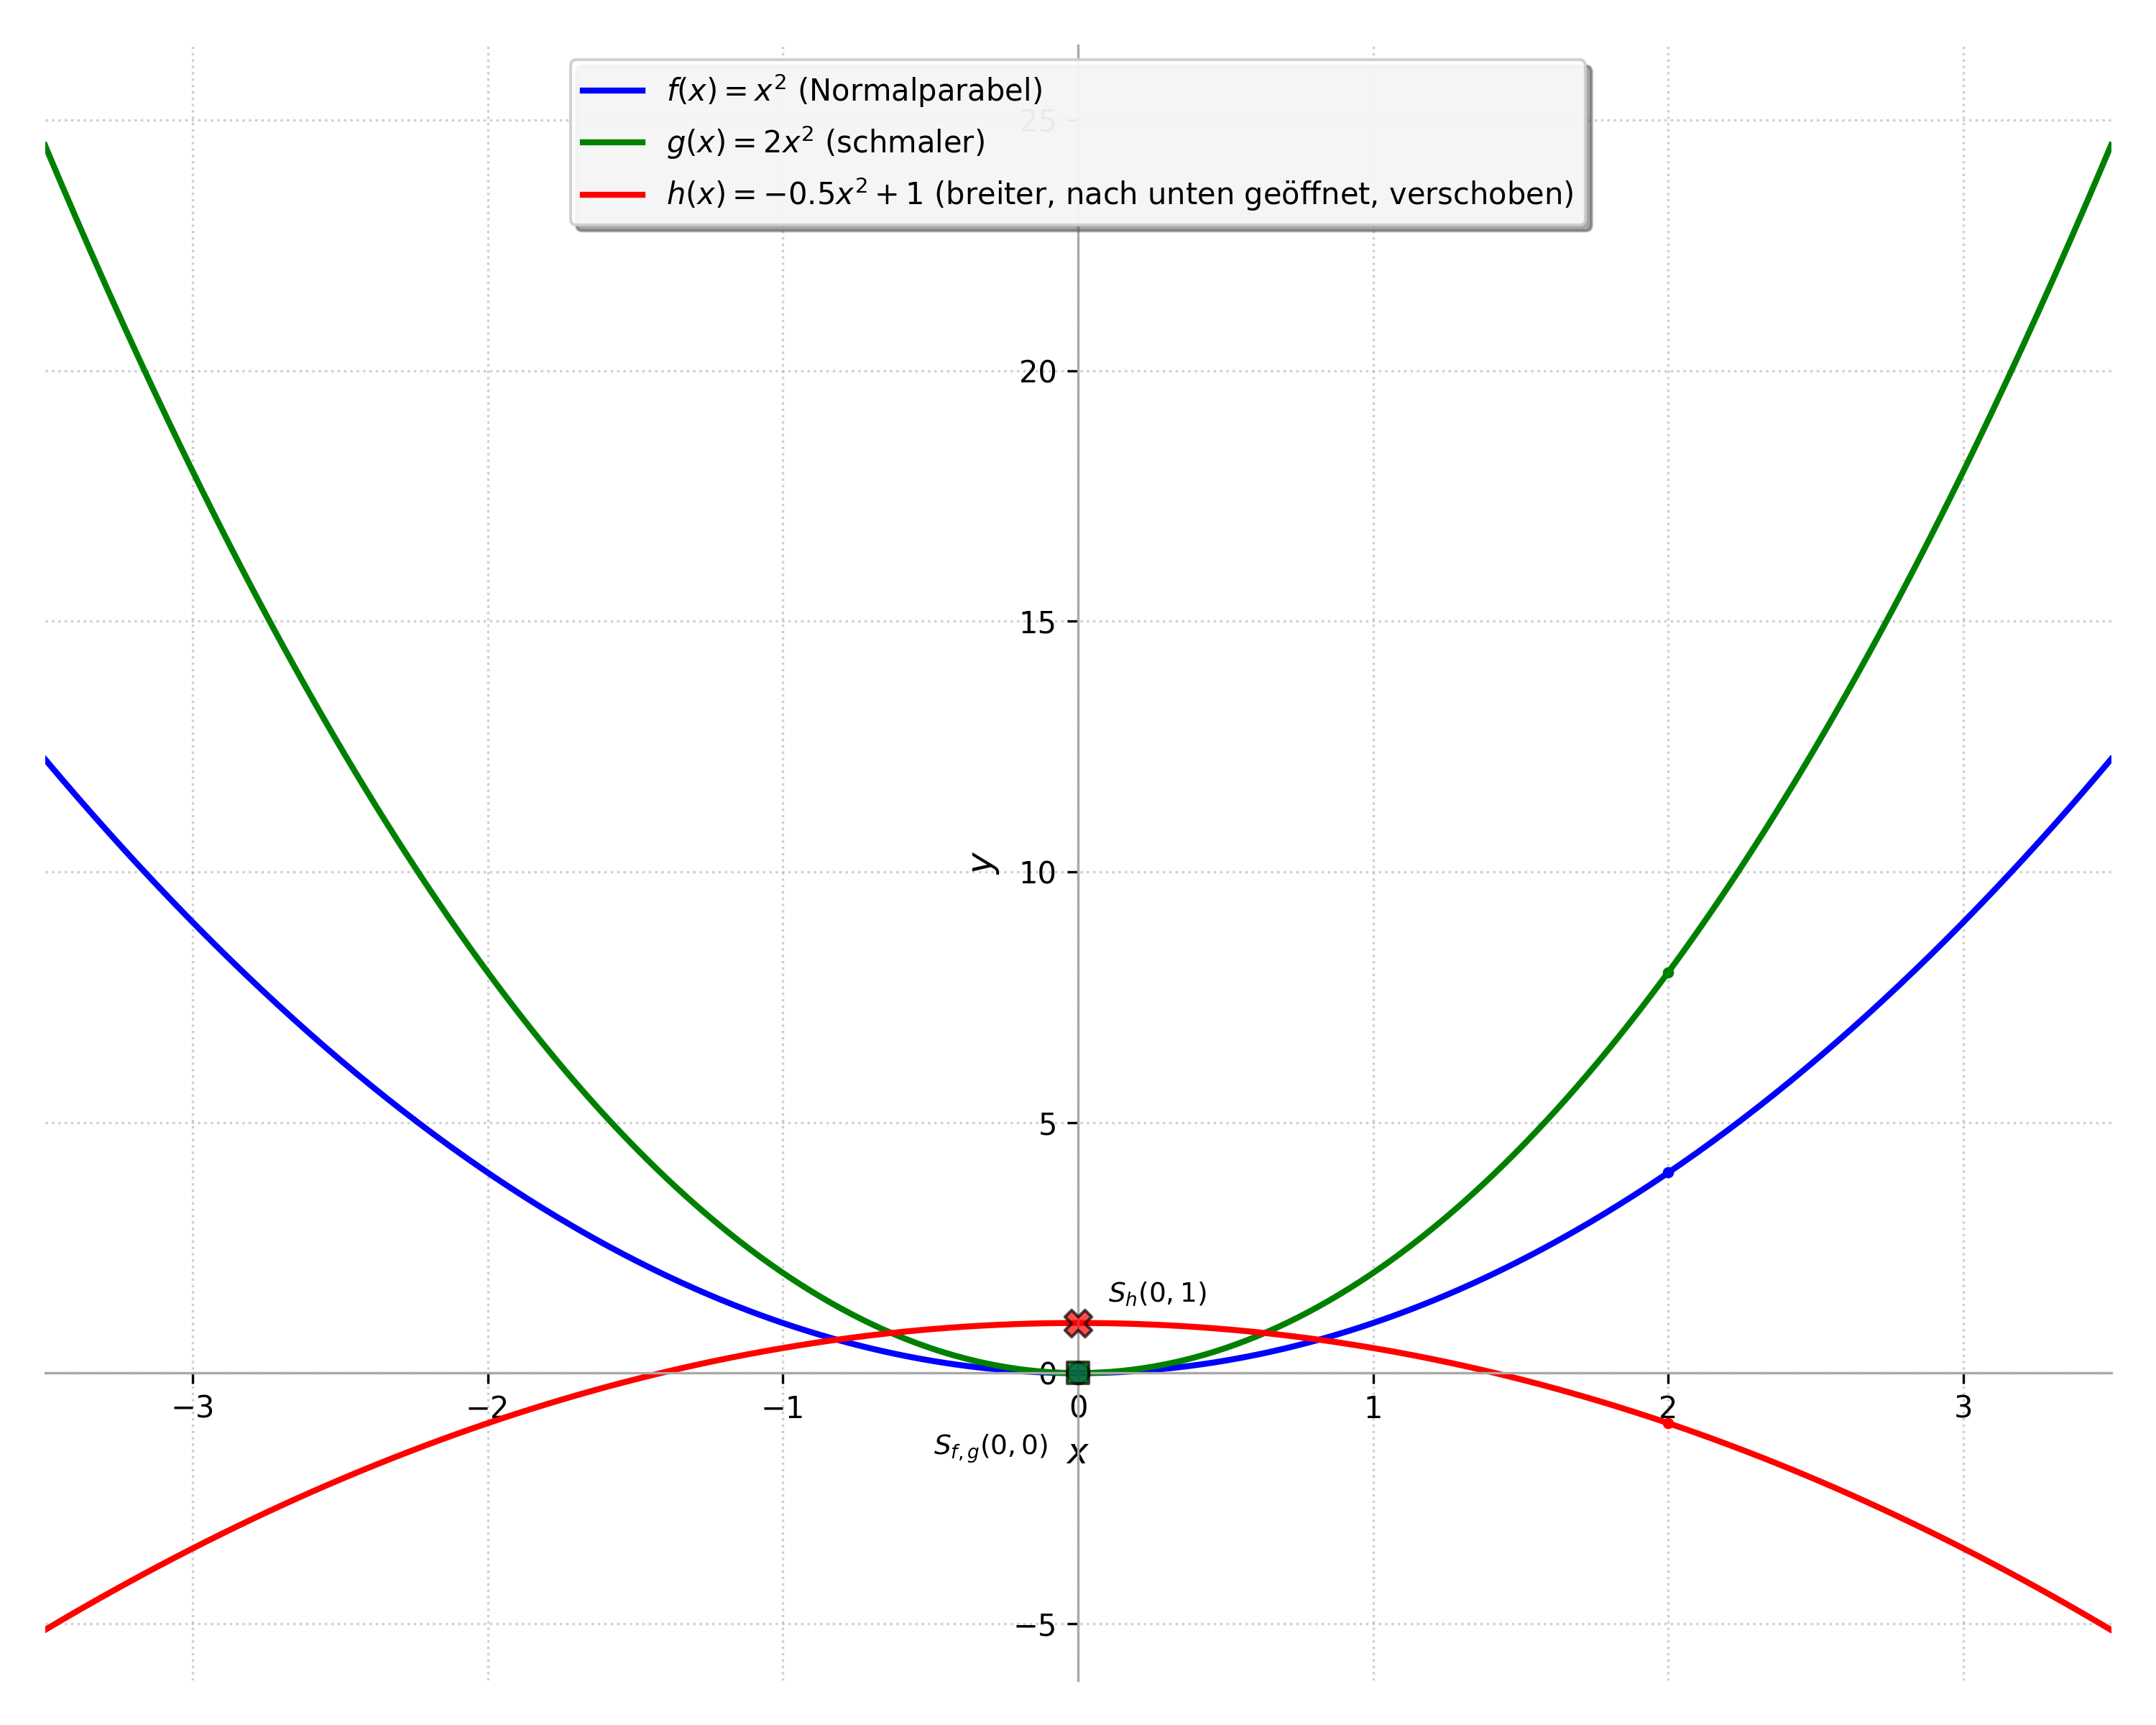
\includegraphics[width=0.8\textwidth]{grafiken/parabeln_vergleich_graph.png}
% --- Beschreibung der Grafik ---
% Die Grafik zeigt ein kartesisches Koordinatensystem.
% Die x-Achse ist beschriftet und skaliert von etwa -4 bis 4.
% Die y-Achse ist beschriftet und skaliert, um alle Funktionswerte abzudecken, z.B. von -5 bis 20.
% Drei Parabeln sind eingezeichnet und idealerweise durch unterschiedliche Farben oder Linienstile gekennzeichnet:
% 1. f(x) = x^2 (Normalparabel): Scheitelpunkt (0|0), nach oben geöffnet, geht durch (1|1), (2|4), (3|9).
% 2. g(x) = 2x^2: Scheitelpunkt (0|0), nach oben geöffnet, schmaler als f(x), geht durch (1|2), (2|8), (3|18).
% 3. h(x) = -0.5x^2 + 1: Scheitelpunkt (0|1), nach unten geöffnet, breiter als f(x), geht durch (1|0.5), (2|-1), (3|-3.5).
% Die Beschriftung der Achsen und der Funktionen (oder ihrer Graphen) ist klar.
\captionof{figure}{Graphen der Funktionen $f(x)=x^2$, $g(x)=2x^2$ und $h(x)=-0.5x^2+1$ im Vergleich.}
\label{fig:parabeln_vergleich}
\end{center}

\end{loesungsumgebung}


\begin{aufgabenumgebung}{Übung zur quadratischen Ergänzung und Scheitelpunktbestimmung}
Bestimme für die folgenden Funktionen den Scheitelpunkt, indem du die Normalform durch quadratische Ergänzung in die Scheitelpunktform überführst. Gib auch an, ob es sich um ein Maximum oder Minimum handelt.
\begin{enumerate}
    \item $f(x) = x^2 - 6x + 5$
    \item $g(x) = x^2 + 8x + 10$
    \item $h(x) = 2x^2 + 4x - 1$ (Tipp: Erst den Faktor 2 ausklammern!)
    \item $k(x) = -x^2 - 2x + 3$ (Tipp: Erst den Faktor -1 ausklammern!)
\end{enumerate}
Vergleiche deine Ergebnisse für $x_S$ mit der Formel $x_S = -b/(2a)$.
\end{aufgabenumgebung}

\begin{loesungsumgebung}[loes:quadratische-ergaenzung-scheitelpunkt]{Übung zur quadratischen Ergänzung und Scheitelpunktbestimmung}
Die Scheitelpunktform einer quadratischen Funktion lautet $f(x) = a(x-x_S)^2 + y_S$, wobei $S(x_S|y_S)$ der Scheitelpunkt der Parabel ist.

\begin{enumerate}[label=(\alph*)]
    \item \textbf{Funktion $f(x) = x^2 - 6x + 5$} \\
    Hier sind $a=1$, $b=-6$, $c=5$.
    \textbf{Quadratische Ergänzung:}
    \begin{align*}
    f(x) &= (x^2 - 6x) + 5 \\
         &= \left(x^2 - 6x + \left(\frac{-6}{2}\right)^2 - \left(\frac{-6}{2}\right)^2\right) + 5 \\
         &= (x^2 - 6x + (-3)^2 - (-3)^2) + 5 \\
         &= (x^2 - 6x + 9) - 9 + 5 \\
         &= (x - 3)^2 - 4
    \end{align*}
    \textbf{Scheitelpunktform:} $f(x) = (x - 3)^2 - 4$. \\
    \textbf{Scheitelpunkt:} $S(3|-4)$. \\
    \textbf{Maximum/Minimum:} Da $a=1 > 0$ (Parabel nach oben geöffnet), handelt es sich um ein \textbf{Minimum}. \\
    \textbf{Vergleich mit Formel $x_S = -b/(2a)$:}
    $x_S = \frac{-(-6)}{2 \cdot 1} = \frac{6}{2} = 3$. Das Ergebnis stimmt mit der quadratischen Ergänzung überein.

    \item \textbf{Funktion $g(x) = x^2 + 8x + 10$} \\
    Hier sind $a=1$, $b=8$, $c=10$.
    \textbf{Quadratische Ergänzung:}
    \begin{align*}
    g(x) &= (x^2 + 8x) + 10 \\
         &= \left(x^2 + 8x + \left(\frac{8}{2}\right)^2 - \left(\frac{8}{2}\right)^2\right) + 10 \\
         &= (x^2 + 8x + 4^2 - 4^2) + 10 \\
         &= (x^2 + 8x + 16) - 16 + 10 \\
         &= (x + 4)^2 - 6
    \end{align*}
    \textbf{Scheitelpunktform:} $g(x) = (x + 4)^2 - 6$. \\
    \textbf{Scheitelpunkt:} $S(-4|-6)$. \\
    \textbf{Maximum/Minimum:} Da $a=1 > 0$ (Parabel nach oben geöffnet), handelt es sich um ein \textbf{Minimum}. \\
    \textbf{Vergleich mit Formel $x_S = -b/(2a)$:}
    $x_S = \frac{-(8)}{2 \cdot 1} = \frac{-8}{2} = -4$. Das Ergebnis stimmt mit der quadratischen Ergänzung überein.

    \item \textbf{Funktion $h(x) = 2x^2 + 4x - 1$} \\
    Hier sind $a=2$, $b=4$, $c=-1$.
    \textbf{Quadratische Ergänzung (Faktor 2 ausklammern):}
    \begin{align*}
    h(x) &= 2(x^2 + 2x) - 1 \\
         &= 2\left(x^2 + 2x + \left(\frac{2}{2}\right)^2 - \left(\frac{2}{2}\right)^2\right) - 1 \\
         &= 2(x^2 + 2x + 1^2 - 1^2) - 1 \\
         &= 2((x^2 + 2x + 1) - 1) - 1 \\
         &= 2(x + 1)^2 - 2 \cdot 1 - 1 \\
         &= 2(x + 1)^2 - 2 - 1 \\
         &= 2(x + 1)^2 - 3
    \end{align*}
    \textbf{Scheitelpunktform:} $h(x) = 2(x + 1)^2 - 3$. \\
    \textbf{Scheitelpunkt:} $S(-1|-3)$. \\
    \textbf{Maximum/Minimum:} Da $a=2 > 0$ (Parabel nach oben geöffnet), handelt es sich um ein \textbf{Minimum}. \\
    \textbf{Vergleich mit Formel $x_S = -b/(2a)$:}
    $x_S = \frac{-(4)}{2 \cdot 2} = \frac{-4}{4} = -1$. Das Ergebnis stimmt mit der quadratischen Ergänzung überein.

    \item \textbf{Funktion $k(x) = -x^2 - 2x + 3$} \\
    Hier sind $a=-1$, $b=-2$, $c=3$.
    \textbf{Quadratische Ergänzung (Faktor -1 ausklammern):}
    \begin{align*}
    k(x) &= -(x^2 + 2x) + 3 \\ % Achten Sie auf das Vorzeichen beim Ausklammern von -1
         &= -\left(x^2 + 2x + \left(\frac{2}{2}\right)^2 - \left(\frac{2}{2}\right)^2\right) + 3 \\
         &= -(x^2 + 2x + 1^2 - 1^2) + 3 \\
         &= -((x^2 + 2x + 1) - 1) + 3 \\
         &= -(x + 1)^2 - (-1) \cdot 1 + 3 \\
         &= -(x + 1)^2 + 1 + 3 \\
         &= -(x + 1)^2 + 4
    \end{align*}
    \textbf{Scheitelpunktform:} $k(x) = -(x + 1)^2 + 4$. \\
    \textbf{Scheitelpunkt:} $S(-1|4)$. \\
    \textbf{Maximum/Minimum:} Da $a=-1 < 0$ (Parabel nach unten geöffnet), handelt es sich um ein \textbf{Maximum}. \\
    \textbf{Vergleich mit Formel $x_S = -b/(2a)$:}
    $x_S = \frac{-(-2)}{2 \cdot (-1)} = \frac{2}{-2} = -1$. Das Ergebnis stimmt mit der quadratischen Ergänzung überein.
\end{enumerate}

\end{loesungsumgebung}


\begin{aufgabenumgebung}{Symmetrie prüfen und bestimmen}
\begin{enumerate}
    \item Untersuche die folgenden Funktionen rechnerisch auf Achsensymmetrie zur y-Achse, indem du $f(-x)$ berechnest und mit $f(x)$ vergleichst.
        \begin{itemize}
            \item $f_1(x) = -3x^2 + 5$
            \item $f_2(x) = x^2 - 2x + 1$
            \item $f_3(x) = 4x^2$
        \end{itemize}
    \item Bestimme für die Funktion $f(x) = 0.5x^2 - 3x + 1$ die Gleichung ihrer Symmetrieachse. Überprüfe dann für zwei verschiedene x-Werte, die symmetrisch zu dieser Achse liegen, ob ihre Funktionswerte gleich sind.
\end{enumerate}
\end{aufgabenumgebung}


\begin{loesungsumgebung}[loes:symmetrie-pruefen-bestimmen]{Symmetrie prüfen und bestimmen}

\begin{enumerate}[label=(\alph*)]
    \item \textbf{Untersuchung auf Achsensymmetrie zur y-Achse} \\
    Eine Funktion $f(x)$ ist achsensymmetrisch zur y-Achse, wenn für alle $x$ aus dem Definitionsbereich gilt: $f(-x) = f(x)$. Dies ist bei quadratischen Funktionen $f(x)=ax^2+bx+c$ genau dann der Fall, wenn der Koeffizient $b=0$ ist (also der lineare Term $bx$ fehlt).

    \begin{itemize}
        \item \textbf{Funktion $f_1(x) = -3x^2 + 5$}
        $$ f_1(-x) = -3(-x)^2 + 5 = -3x^2 + 5 $$
        Da $f_1(-x) = -3x^2 + 5 = f_1(x)$ ist, ist die Funktion $f_1(x)$ \textbf{achsensymmetrisch zur y-Achse}. (Hier ist $b=0$).

        \item \textbf{Funktion $f_2(x) = x^2 - 2x + 1$}
        $$ f_2(-x) = (-x)^2 - 2(-x) + 1 = x^2 + 2x + 1 $$
        Da $f_2(-x) = x^2 + 2x + 1 \neq x^2 - 2x + 1 = f_2(x)$ (für $x \neq 0$), ist die Funktion $f_2(x)$ \textbf{nicht achsensymmetrisch zur y-Achse}. (Hier ist $b=-2 \neq 0$).

        \item \textbf{Funktion $f_3(x) = 4x^2$}
        $$ f_3(-x) = 4(-x)^2 = 4x^2 $$
        Da $f_3(-x) = 4x^2 = f_3(x)$ ist, ist die Funktion $f_3(x)$ \textbf{achsensymmetrisch zur y-Achse}. (Hier ist $b=0$ und $c=0$).
    \end{itemize}

    \item \textbf{Bestimmung der Symmetrieachse für $f(x) = 0.5x^2 - 3x + 1$} \\
    Die Symmetrieachse einer Parabel mit der Gleichung $f(x) = ax^2+bx+c$ ist eine vertikale Gerade mit der Gleichung $x = x_S = \frac{-b}{2a}$.
    Für die gegebene Funktion $f(x) = 0.5x^2 - 3x + 1$ sind die Koeffizienten:
    $a = 0.5$, $b = -3$, $c = 1$.

    Berechnung von $x_S$:
    $$ x_S = \frac{-(-3)}{2 \cdot 0.5} = \frac{3}{1} = 3 $$
    Die Gleichung der \textbf{Symmetrieachse ist $x = 3$}.

    \textbf{Überprüfung der Symmetrie:}
    Wir wählen zwei $x$-Werte, die symmetrisch zur Achse $x=3$ liegen. Das bedeutet, sie haben den gleichen Abstand $d$ von der Achse $x=3$.
    Sei z.B. der Abstand $d=1$:
    \begin{itemize}
        \item $x_1 = x_S - d = 3 - 1 = 2$
        \item $x_2 = x_S + d = 3 + 1 = 4$
    \end{itemize}
    Nun berechnen wir die Funktionswerte an diesen Stellen:
    \begin{itemize}
        \item $f(x_1) = f(2) = 0.5(2)^2 - 3(2) + 1 = 0.5 \cdot 4 - 6 + 1 = 2 - 6 + 1 = -3$.
        \item $f(x_2) = f(4) = 0.5(4)^2 - 3(4) + 1 = 0.5 \cdot 16 - 12 + 1 = 8 - 12 + 1 = -3$.
    \end{itemize}
    Da $f(2) = -3$ und $f(4) = -3$ ist, sind die Funktionswerte gleich ($f(x_S-d) = f(x_S+d)$).

    Wählen wir einen anderen Abstand, z.B. $d=2$:
    \begin{itemize}
        \item $x_3 = x_S - d = 3 - 2 = 1$
        \item $x_4 = x_S + d = 3 + 2 = 5$
    \end{itemize}
    Funktionswerte:
    \begin{itemize}
        \item $f(x_3) = f(1) = 0.5(1)^2 - 3(1) + 1 = 0.5 \cdot 1 - 3 + 1 = 0.5 - 3 + 1 = -1.5$.
        \item $f(x_4) = f(5) = 0.5(5)^2 - 3(5) + 1 = 0.5 \cdot 25 - 15 + 1 = 12.5 - 15 + 1 = -1.5$.
    \end{itemize}
    Auch hier sind die Funktionswerte $f(1) = -1.5$ und $f(5) = -1.5$ gleich.
    Die Überprüfung bestätigt, dass $x=3$ die Symmetrieachse der Funktion $f(x)$ ist.
\end{enumerate}

\end{loesungsumgebung}



\begin{aufgabenumgebung}{Nullstellen finden – Übung und Vertiefung}
Berechne die Nullstellen der folgenden Funktionen. Entscheide selbst, welche Methode (Ausklammern, p-q-Formel, Mitternachtsformel, Substitution) am besten geeignet ist. Überprüfe bei quadratischen Gleichungen immer zuerst die Diskriminante, um die Anzahl der erwarteten reellen Nullstellen zu bestimmen.
\begin{enumerate}
    \item $f(x) = x^2 - x - 6$


    \item $g(x) = -2x^2 + 12x - 18$ 


    \item $h(x) = x^2 + 2x + 5$


    \item $k(x) = 3x^2 - 12$ 


    \item $m(x) = -0.5x^2 + 2x$


    \item \textbf{Polynom 3. Grades durch Ausklammern:}
        $p(x) = x^3 - 5x^2 + 6x$


    \item \textbf{Biquadratische Funktion:}
        $q(x) = x^4 - 10x^2 + 9$


    \item \textbf{Produkt aus Linearfaktoren (versteckt):}
        $r(x) = (x^2-4)(x^2+x-2)$


    \item \textbf{Funktion mit bekannter Nullstelle (für Knobler):}
        Gegeben ist die Funktion $s(x) = x^3 - 2x^2 - 5x + 6$. Es ist bekannt, dass $x_1=1$ eine Nullstelle ist. Finde die anderen Nullstellen.



    \item \textbf{Nullstellen und Parameter:}
        Für welche Werte des Parameters $k$ hat die Funktion $f_k(x) = x^2 - 2kx + (k+2)$ genau eine, zwei oder keine reelle(n) Nullstelle(n)?


\end{enumerate}
\end{aufgabenumgebung}


\begin{loesungsumgebung}[loes:nullstellen-uebung-vertiefung]{Nullstellen finden – Übung und Vertiefung}
Um die Nullstellen einer Funktion $f(x)$ zu finden, setzen wir $f(x)=0$ und lösen die entstehende Gleichung nach $x$.

\begin{enumerate}[label=(\alph*)]
    \item \textbf{Funktion $f(x) = x^2 - x - 6$} \\
    Dies ist eine quadratische Gleichung in der Normalform $ax^2+bx+c=0$ mit $a=1, b=-1, c=-6$. Wir verwenden die Mitternachtsformel (oder p-q-Formel, da $a=1$).
    \textbf{Diskriminante:} $D = b^2 - 4ac = (-1)^2 - 4(1)(-6) = 1 + 24 = 25$.
    Da $D > 0$, gibt es zwei verschiedene reelle Nullstellen.
    \textbf{Nullstellenberechnung (Mitternachtsformel):}
    $$ x_{1,2} = \frac{-b \pm \sqrt{D}}{2a} = \frac{-(-1) \pm \sqrt{25}}{2(1)} = \frac{1 \pm 5}{2} $$
    $$ x_1 = \frac{1+5}{2} = \frac{6}{2} = 3 $$
    $$ x_2 = \frac{1-5}{2} = \frac{-4}{2} = -2 $$
    Die Nullstellen sind $x_1=3$ und $x_2=-2$.

    \item \textbf{Funktion $g(x) = -2x^2 + 12x - 18$} \\
    Quadratische Gleichung mit $a=-2, b=12, c=-18$.
    \textbf{Diskriminante:} $D = b^2 - 4ac = (12)^2 - 4(-2)(-18) = 144 - 144 = 0$.
    \textbf{Anmerkung zur Diskriminante (Tipp):} Da $D=0$, gibt es genau eine (doppelte) reelle Nullstelle. Der Scheitelpunkt der Parabel liegt auf der x-Achse, d.h., der Graph berührt die x-Achse an dieser Stelle.
    \textbf{Nullstellenberechnung (Mitternachtsformel):}
    $$ x_0 = \frac{-b \pm \sqrt{D}}{2a} = \frac{-12 \pm \sqrt{0}}{2(-2)} = \frac{-12}{-4} = 3 $$
    Die Nullstelle ist $x_0=3$ (doppelte Nullstelle).

    \item \textbf{Funktion $h(x) = x^2 + 2x + 5$} \\
    Quadratische Gleichung mit $a=1, b=2, c=5$.
    \textbf{Diskriminante:} $D = b^2 - 4ac = (2)^2 - 4(1)(5) = 4 - 20 = -16$.
    \textbf{Anmerkung zur Diskriminante (Tipp):} Da $D < 0$, gibt es keine reellen Nullstellen. Der Graph der Parabel schneidet die x-Achse nicht. Da $a=1>0$ (Parabel nach oben geöffnet), verläuft der Graph vollständig oberhalb der x-Achse.
    Die Funktion $h(x)$ hat keine reellen Nullstellen.

    \item \textbf{Funktion $k(x) = 3x^2 - 12$} \\
    Setze $k(x)=0$: $3x^2 - 12 = 0$. Diese reinquadratische Gleichung lässt sich direkt auflösen.
    \textbf{Umformungsschritte:}
    $$
    \begin{array}{r c l c l}
    \umformung{3x^2 - 12}{0}{+}{12}
    \umformung{3x^2}{12}{\div}{3}
    \umformungend{x^2}{4}
    \end{array}
    $$
    Aus $x^2=4$ folgt durch Wurzelziehen: $x = \pm\sqrt{4}$.
    Die Nullstellen sind $x_1=2$ und $x_2=-2$.

    \item \textbf{Funktion $m(x) = -0.5x^2 + 2x$} \\
    Setze $m(x)=0$: $-0.5x^2 + 2x = 0$. Hier fehlt der konstante Term ($c=0$), daher ist Ausklammern geeignet.
    \textbf{Ausklammern:}
    $$ x(-0.5x + 2) = 0 $$
    Nach dem Satz vom Nullprodukt ist ein Produkt genau dann Null, wenn mindestens einer der Faktoren Null ist:
    \begin{enumerate}
        \item $x_1 = 0$
        \item $-0.5x + 2 = 0$
            $$
            \begin{array}{r c l c l}
            \umformung{-0.5x + 2}{0}{-}{2}
            \umformung{-0.5x}{-2}{\div}{(-0.5)}
            \umformungend{x_2}{4}
            \end{array}
            $$
    \end{enumerate}
    Die Nullstellen sind $x_1=0$ und $x_2=4$.

    \item \textbf{Polynom 3. Grades durch Ausklammern: $p(x) = x^3 - 5x^2 + 6x$} \\
    Setze $p(x)=0$: $x^3 - 5x^2 + 6x = 0$.
    \textbf{Strategie (Tipp):} Klammere den gemeinsamen Faktor $x$ aus.
    $$ x(x^2 - 5x + 6) = 0 $$
    Nach dem Satz vom Nullprodukt:
    \begin{enumerate}
        \item $x_1 = 0$
        \item $x^2 - 5x + 6 = 0$ (Quadratische Gleichung) \\
        Hier $a=1, b=-5, c=6$.
        Diskriminante: $D = (-5)^2 - 4(1)(6) = 25 - 24 = 1$.
        $x_{2,3} = \frac{-(-5) \pm \sqrt{1}}{2(1)} = \frac{5 \pm 1}{2}$.
        $x_2 = \frac{5+1}{2} = 3$.
        $x_3 = \frac{5-1}{2} = 2$.
    \end{enumerate}
    Die Nullstellen sind $x_1=0$, $x_2=3$ und $x_3=2$.

    \item \textbf{Biquadratische Funktion: $q(x) = x^4 - 10x^2 + 9$} \\
    Setze $q(x)=0$: $x^4 - 10x^2 + 9 = 0$.
    \textbf{Strategie (Tipp):} Substitution $z = x^2$. Dann ist $z^2 = x^4$.
    Die Gleichung wird zu einer quadratischen Gleichung in $z$:
    $$ z^2 - 10z + 9 = 0 $$
    Lösen für $z$ (mit $a=1, b=-10, c=9$):
    Diskriminante: $D_z = (-10)^2 - 4(1)(9) = 100 - 36 = 64$.
    $z_{1,2} = \frac{-(-10) \pm \sqrt{64}}{2(1)} = \frac{10 \pm 8}{2}$.
    $z_1 = \frac{10+8}{2} = 9$.
    $z_2 = \frac{10-8}{2} = 1$.
    \textbf{Rücksubstitution:}
    \begin{itemize}
        \item Für $z_1 = 9$: $x^2 = 9 \implies x = \pm\sqrt{9} \implies x_{1,2} = \pm 3$.
        \item Für $z_2 = 1$: $x^2 = 1 \implies x = \pm\sqrt{1} \implies x_{3,4} = \pm 1$.
    \end{itemize}
    (Beide $z$-Werte sind positiv, daher führen sie zu reellen $x$-Lösungen).
    Die Nullstellen sind $x_1=3$, $x_2=-3$, $x_3=1$ und $x_4=-1$.

    \item \textbf{Produkt aus Linearfaktoren (versteckt): $r(x) = (x^2-4)(x^2+x-2)$} \\
    Setze $r(x)=0$: $(x^2-4)(x^2+x-2) = 0$.
    \textbf{Strategie (Tipp):} Nach dem Satz vom Nullprodukt setzen wir jeden Faktor gleich Null.
    \begin{enumerate}
        \item Faktor 1: $x^2-4 = 0$
            $$ x^2 = 4 \implies x = \pm\sqrt{4} \implies x_{1,2} = \pm 2 $$
            (Also $x_1=2, x_2=-2$)
        \item Faktor 2: $x^2+x-2 = 0$ \\
            Hier $a=1, b=1, c=-2$.
            Diskriminante: $D = (1)^2 - 4(1)(-2) = 1 + 8 = 9$.
            $x_{3,4} = \frac{-1 \pm \sqrt{9}}{2(1)} = \frac{-1 \pm 3}{2}$.
            $x_3 = \frac{-1+3}{2} = 1$.
            $x_4 = \frac{-1-3}{2} = -2$.
    \end{enumerate}
    Die Menge der Nullstellen ist $\{2, -2, 1\}$. Die Nullstelle $x=-2$ tritt in beiden Faktoren auf (ist eine mehrfache Nullstelle des Gesamtpolynoms). Die verschiedenen Nullstellen sind $x_1=2$, $x_2=-2$ und $x_3=1$.

    \item \textbf{Funktion mit bekannter Nullstelle (für Knobler): $s(x) = x^3 - 2x^2 - 5x + 6$} \\
    Gegeben ist $x_1=1$ als Nullstelle.
    \textbf{Strategie (Tipp):} Koeffizientenvergleich. Wenn $x_1=1$ eine Nullstelle ist, dann ist $(x-1)$ ein Linearfaktor. Wir suchen $ax^2+bx+c$, sodass $s(x)=(x-1)(ax^2+bx+c)$.
    Aus dem Tipp ergibt sich $a=1, c=-6, b=-1$. Der quadratische Faktor ist also $(x^2-x-6)$.
    Wir müssen nun die Nullstellen dieses quadratischen Faktors finden:
    $$ x^2-x-6=0 $$
    Diese Gleichung wurde bereits in Teil (a) gelöst. Die Nullstellen sind $x=3$ und $x=-2$.
    Die Nullstellen der Funktion $s(x)$ sind also $x_1=1$, $x_2=3$ und $x_3=-2$.

    \item \textbf{Nullstellen und Parameter: $f_k(x) = x^2 - 2kx + (k+2)$} \\
    Wir untersuchen die Diskriminante $D = B^2-4AC$ der quadratischen Gleichung $f_k(x)=0$. Hier sind $A=1$, $B=-2k$, $C=(k+2)$.
    $$ D = (-2k)^2 - 4(1)(k+2) = 4k^2 - 4(k+2) = 4k^2 - 4k - 8 $$
    \begin{itemize}
        \item \textbf{Genau eine reelle Nullstelle:} $D=0$.
        $$ 4k^2 - 4k - 8 = 0 $$
        Teilen durch 4:
        $$ k^2 - k - 2 = 0 $$
        Lösen für $k$ (mit $a_k=1, b_k=-1, c_k=-2$):
        $D_k = (-1)^2 - 4(1)(-2) = 1+8=9$.
        $k_{1,2} = \frac{-(-1) \pm \sqrt{9}}{2(1)} = \frac{1 \pm 3}{2}$.
        $k_1 = \frac{1+3}{2} = 2$.
        $k_2 = \frac{1-3}{2} = -1$.
        Für $k=2$ oder $k=-1$ hat die Funktion $f_k(x)$ genau eine reelle Nullstelle.
        \item \textbf{Zwei verschiedene reelle Nullstellen:} $D>0$.
        $$ 4k^2 - 4k - 8 > 0 \implies k^2 - k - 2 > 0 $$
        Die Parabel $P(k) = k^2 - k - 2$ ist nach oben geöffnet und hat Nullstellen bei $k=-1$ und $k=2$. Sie ist positiv für Werte außerhalb ihrer Nullstellen.
        Also für $k < -1$ oder $k > 2$. In Intervallschreibweise: $k \in (-\infty, -1) \cup (2, \infty)$.
        \item \textbf{Keine reelle(n) Nullstelle(n):} $D<0$.
        $$ 4k^2 - 4k - 8 < 0 \implies k^2 - k - 2 < 0 $$
        Die Parabel $P(k) = k^2 - k - 2$ ist negativ für Werte zwischen ihren Nullstellen.
        Also für $-1 < k < 2$. In Intervallschreibweise: $k \in (-1, 2)$.
    \end{itemize}
\end{enumerate}

\end{loesungsumgebung}



\begin{aufgabenumgebung}
        \textbf{Anwendung des Satzes von Vieta (Kopfrechnen für Profis):}
        Versuche, die Nullstellen der folgenden quadratischen Funktionen (in Normalform $x^2+px+q=0$) durch 'scharfes Hinsehen' mit dem Satz von Vieta zu finden. Suche also zwei Zahlen $x_1, x_2$, für die gilt: $x_1+x_2 = -p$ und $x_1 \cdot x_2 = q$.
        \begin{enumerate}[label=(\alph*)]
            \item $f(x) = x^2 - 5x + 6$
            \item $g(x) = x^2 - 3x - 4$
            \item $h(x) = x^2 + 7x + 10$
        \end{enumerate}
\end{aufgabenumgebung}


\begin{loesungsumgebung}[loes:satz-von-vieta]{Anwendung des Satzes von Vieta (Kopfrechnen für Profis)}
Der Satz von Vieta bietet eine elegante Methode, um die Nullstellen einer quadratischen Funktion der Form $f(x) = x^2+px+q$ zu finden, sofern diese ganzzahlig (oder leicht zu erraten) sind. Man sucht zwei Zahlen $x_1$ und $x_2$, für die gilt:
\begin{itemize}
    \item $x_1 + x_2 = -p$
    \item $x_1 \cdot x_2 = q$
\end{itemize}
Diese Zahlen $x_1$ und $x_2$ sind dann die Nullstellen der Funktion.

\begin{enumerate}[label=(\alph*)]
    \item \textbf{Funktion $f(x) = x^2 - 5x + 6$} \\
    Hier ist $p=-5$ und $q=6$.
    Wir suchen zwei Zahlen $x_1, x_2$, für die gilt:
    \begin{itemize}
        \item $x_1 + x_2 = -(-5) = 5$
        \item $x_1 \cdot x_2 = 6$
    \end{itemize}
    Wir betrachten die ganzzahligen Teiler von $q=6$: $\pm 1, \pm 2, \pm 3, \pm 6$.
    Mögliche Paare für das Produkt $x_1 \cdot x_2 = 6$:
    \begin{itemize}
        \item $1 \cdot 6 = 6 \implies 1+6 = 7 \neq 5$
        \item $2 \cdot 3 = 6 \implies 2+3 = 5$ \textbf{(Treffer!)}
        \item $(-1) \cdot (-6) = 6 \implies (-1)+(-6) = -7 \neq 5$
        \item $(-2) \cdot (-3) = 6 \implies (-2)+(-3) = -5 \neq 5$
    \end{itemize}
    Die gesuchten Zahlen sind $2$ und $3$.
    Die Nullstellen sind also $x_1 = 2$ und $x_2 = 3$.

    \item \textbf{Funktion $g(x) = x^2 - 3x - 4$} \\
    Hier ist $p=-3$ und $q=-4$.
    Wir suchen zwei Zahlen $x_1, x_2$, für die gilt:
    \begin{itemize}
        \item $x_1 + x_2 = -(-3) = 3$
        \item $x_1 \cdot x_2 = -4$
    \end{itemize}
    Da das Produkt $q=-4$ negativ ist, müssen die beiden Zahlen unterschiedliche Vorzeichen haben.
    Mögliche Paare für das Produkt $x_1 \cdot x_2 = -4$:
    \begin{itemize}
        \item $1 \cdot (-4) = -4 \implies 1+(-4) = -3 \neq 3$
        \item $(-1) \cdot 4 = -4 \implies (-1)+4 = 3$ \textbf{(Treffer!)}
        \item $2 \cdot (-2) = -4 \implies 2+(-2) = 0 \neq 3$
    \end{itemize}
    Die gesuchten Zahlen sind $-1$ und $4$.
    Die Nullstellen sind also $x_1 = -1$ und $x_2 = 4$.

    \item \textbf{Funktion $h(x) = x^2 + 7x + 10$} \\
    Hier ist $p=7$ und $q=10$.
    Wir suchen zwei Zahlen $x_1, x_2$, für die gilt:
    \begin{itemize}
        \item $x_1 + x_2 = -(7) = -7$
        \item $x_1 \cdot x_2 = 10$
    \end{itemize}
    Da das Produkt $q=10$ positiv ist und die Summe $x_1+x_2=-7$ negativ ist, müssen beide Zahlen negativ sein.
    Mögliche Paare (negative Teiler von 10):
    \begin{itemize}
        \item $(-1) \cdot (-10) = 10 \implies (-1)+(-10) = -11 \neq -7$
        \item $(-2) \cdot (-5) = 10 \implies (-2)+(-5) = -7$ \textbf{(Treffer!)}
    \end{itemize}
    Die gesuchten Zahlen sind $-2$ und $-5$.
    Die Nullstellen sind also $x_1 = -2$ und $x_2 = -5$.
\end{enumerate}

\end{loesungsumgebung}


\begin{aufgabenumgebung}{Deine Kurvendiskussion – Quadratische Funktionen}
Führe eine vollständige Kurvendiskussion (gemäß der obigen Checkliste) für die folgenden quadratischen Funktionen durch und skizziere jeweils den Graphen.
\begin{enumerate}
    \item $f(x) = x^2 - 4x + 3$
    \item $g(x) = -2x^2 + 8x - 6$
    \item $h(x) = x^2 + 2x + 2$ (Was ist hier bei den Nullstellen und dem Scheitelpunkt besonders?)
    \item $k(x) = x^2 - 2x + 3$ (Untersuche, ob diese Funktion Nullstellen besitzt. Wie wirkt sich das auf den Graphen und den Wertebereich aus?)
    \item $m(x) = -x^2 - 3x + 4$ (Achte auf die Vorzeichen bei der Berechnung des Scheitelpunkts und der Nullstellen.)
\end{enumerate}
\end{aufgabenumgebung}



\begin{loesungsumgebung}[loes:kurvendiskussion-quadratisch]{Deine Kurvendiskussion – Quadratische Funktionen}
Wir führen für jede der gegebenen quadratischen Funktionen eine vollständige Kurvendiskussion gemäß der Checkliste durch.

\subsection*{1. Kurvendiskussion von $f(x) = x^2 - 4x + 3$}
\begin{enumerate}[label=(\alph*)]
    \item \textbf{Grundlegende Eigenschaften und Definitionsbereich $D_f$:}
    \begin{itemize}
        \item Koeffizienten: $a=1, b=-4, c=3$.
        \item Öffnungsrichtung: Da $a=1 > 0$, ist die Parabel nach \textbf{oben geöffnet}.
        \item Form: Da $|a|=|1|=1$, hat die Parabel die \textbf{Normalform} (Standardöffnung).
        \item Definitionsbereich: $D_f = \mathbb{R}$.
    \end{itemize}
    \item \textbf{Symmetrie:}
    Die Parabel ist achsensymmetrisch zur senkrechten Geraden $x = x_S$. Die genaue Lage von $x_S$ wird beim Scheitelpunkt berechnet. Da $b=-4 \neq 0$, ist die Parabel nicht achsensymmetrisch zur y-Achse.
    \item \textbf{Verhalten für $x \to \pm \infty$ (Globalverhalten):}
    Da $a=1 > 0$:
    \begin{itemize}
        \item $f(x) \to \infty$ für $x \to \infty$.
        \item $f(x) \to \infty$ für $x \to -\infty$.
    \end{itemize}
    \item \textbf{Schnittpunkt mit der y-Achse ($P_y$):}
    $f(0) = (0)^2 - 4(0) + 3 = 3$. Der Punkt ist $P_y(0|3)$.
    \item \textbf{Nullstellen (Schnittpunkte mit der x-Achse, $N_1, N_2$):}
    Setze $f(x)=0 \Rightarrow x^2 - 4x + 3 = 0$.
    Diskriminante: $D = b^2 - 4ac = (-4)^2 - 4(1)(3) = 16 - 12 = 4$.
    Da $D=4 > 0$, gibt es zwei verschiedene reelle Nullstellen.
    $x_{1,2} = \frac{-b \pm \sqrt{D}}{2a} = \frac{-(-4) \pm \sqrt{4}}{2(1)} = \frac{4 \pm 2}{2}$.
    $x_1 = \frac{4+2}{2} = 3$.
    $x_2 = \frac{4-2}{2} = 1$.
    Die Nullstellenpunkte sind $N_1(3|0)$ und $N_2(1|0)$.
    \item \textbf{Scheitelpunkt $S(x_S|y_S)$ (Extrempunkt):}
    $x_S = -\frac{b}{2a} = -\frac{-4}{2(1)} = \frac{4}{2} = 2$.
    $y_S = f(x_S) = f(2) = (2)^2 - 4(2) + 3 = 4 - 8 + 3 = -1$.
    Scheitelpunkt $S(2|-1)$. Da $a=1 > 0$, ist dies ein \textbf{Tiefpunkt (Minimum)}.
    Die Symmetrieachse ist die Gerade $x=2$.
    \item \textbf{Wertebereich $W_f$:}
    Da $a>0$ und der Tiefpunkt bei $y_S=-1$ liegt: $W_f = \{ y \in \mathbb{R} \,|\, y \ge -1 \} = [-1, \infty)$.
\end{enumerate}

\subsection*{2. Kurvendiskussion von $g(x) = -2x^2 + 8x - 6$}
\begin{enumerate}[label=(\alph*)]
    \item \textbf{Grundlegende Eigenschaften und Definitionsbereich $D_g$:}
    \begin{itemize}
        \item Koeffizienten: $a=-2, b=8, c=-6$.
        \item Öffnungsrichtung: Da $a=-2 < 0$, ist die Parabel nach \textbf{unten geöffnet}.
        \item Form: Da $|a|=|-2|=2 > 1$, ist die Parabel \textbf{schmaler} als die Normalparabel (gestreckt).
        \item Definitionsbereich: $D_g = \mathbb{R}$.
    \end{itemize}
    \item \textbf{Symmetrie:}
    Symmetrieachse $x = x_S$. Da $b=8 \neq 0$, nicht symmetrisch zur y-Achse.
    \item \textbf{Verhalten für $x \to \pm \infty$:}
    Da $a=-2 < 0$:
    \begin{itemize}
        \item $g(x) \to -\infty$ für $x \to \infty$.
        \item $g(x) \to -\infty$ für $x \to -\infty$.
    \end{itemize}
    \item \textbf{Schnittpunkt mit der y-Achse ($P_y$):}
    $g(0) = -2(0)^2 + 8(0) - 6 = -6$. Der Punkt ist $P_y(0|-6)$.
    \item \textbf{Nullstellen ($N_1, N_2$):}
    Setze $g(x)=0 \Rightarrow -2x^2 + 8x - 6 = 0$.
    Diskriminante: $D = b^2 - 4ac = (8)^2 - 4(-2)(-6) = 64 - 48 = 16$.
    Da $D=16 > 0$, gibt es zwei verschiedene reelle Nullstellen.
    $x_{1,2} = \frac{-b \pm \sqrt{D}}{2a} = \frac{-8 \pm \sqrt{16}}{2(-2)} = \frac{-8 \pm 4}{-4}$.
    $x_1 = \frac{-8+4}{-4} = \frac{-4}{-4} = 1$.
    $x_2 = \frac{-8-4}{-4} = \frac{-12}{-4} = 3$.
    Die Nullstellenpunkte sind $N_1(1|0)$ und $N_2(3|0)$.
    \item \textbf{Scheitelpunkt $S(x_S|y_S)$ (Extrempunkt):}
    $x_S = -\frac{b}{2a} = -\frac{8}{2(-2)} = -\frac{8}{-4} = 2$.
    $y_S = g(x_S) = g(2) = -2(2)^2 + 8(2) - 6 = -2(4) + 16 - 6 = -8 + 16 - 6 = 2$.
    Scheitelpunkt $S(2|2)$. Da $a=-2 < 0$, ist dies ein \textbf{Hochpunkt (Maximum)}.
    Die Symmetrieachse ist die Gerade $x=2$.
    \item \textbf{Wertebereich $W_g$:}
    Da $a<0$ und der Hochpunkt bei $y_S=2$ liegt: $W_g = \{ y \in \mathbb{R} \,|\, y \le 2 \} = (-\infty, 2]$.
\end{enumerate}

\subsection*{3. Kurvendiskussion von $h(x) = x^2 + 2x + 2$}
\begin{enumerate}[label=(\alph*)]
    \item \textbf{Grundlegende Eigenschaften und Definitionsbereich $D_h$:}
    \begin{itemize}
        \item Koeffizienten: $a=1, b=2, c=2$.
        \item Öffnungsrichtung: Da $a=1 > 0$, ist die Parabel nach \textbf{oben geöffnet}.
        \item Form: Da $|a|=|1|=1$, hat die Parabel die \textbf{Normalform}.
        \item Definitionsbereich: $D_h = \mathbb{R}$.
    \end{itemize}
    \item \textbf{Symmetrie:}
    Symmetrieachse $x = x_S$. Da $b=2 \neq 0$, nicht symmetrisch zur y-Achse.
    \item \textbf{Verhalten für $x \to \pm \infty$:}
    Da $a=1 > 0$: $h(x) \to \infty$ für $x \to \pm \infty$.
    \item \textbf{Schnittpunkt mit der y-Achse ($P_y$):}
    $h(0) = (0)^2 + 2(0) + 2 = 2$. Der Punkt ist $P_y(0|2)$.
    \item \textbf{Nullstellen:}
    Setze $h(x)=0 \Rightarrow x^2 + 2x + 2 = 0$.
    Diskriminante: $D = b^2 - 4ac = (2)^2 - 4(1)(2) = 4 - 8 = -4$.
    Da $D < 0$, gibt es \textbf{keine reellen Nullstellen}.
    \item \textbf{Scheitelpunkt $S(x_S|y_S)$ (Extrempunkt):}
    $x_S = -\frac{b}{2a} = -\frac{2}{2(1)} = -1$.
    $y_S = h(x_S) = h(-1) = (-1)^2 + 2(-1) + 2 = 1 - 2 + 2 = 1$.
    Scheitelpunkt $S(-1|1)$. Da $a=1 > 0$, ist dies ein \textbf{Tiefpunkt (Minimum)}.
    Die Symmetrieachse ist die Gerade $x=-1$.
    \textit{Anmerkung (Was ist hier bei den Nullstellen und dem Scheitelpunkt besonders?):} Die Funktion hat keine reellen Nullstellen. Der Scheitelpunkt $S(-1|1)$ liegt oberhalb der x-Achse ($y_S=1 > 0$), und da die Parabel nach oben geöffnet ist, schneidet sie die x-Achse nicht. Der y-Wert des Scheitelpunkts ist der kleinste Funktionswert.
    \item \textbf{Wertebereich $W_h$:}
    Da $a>0$ und der Tiefpunkt bei $y_S=1$ liegt: $W_h = [1, \infty)$.
\end{enumerate}

\subsection*{4. Kurvendiskussion von $k(x) = x^2 - 2x + 3$}
\begin{enumerate}[label=(\alph*)]
    \item \textbf{Grundlegende Eigenschaften und Definitionsbereich $D_k$:}
    \begin{itemize}
        \item Koeffizienten: $a=1, b=-2, c=3$.
        \item Öffnungsrichtung: Da $a=1 > 0$, ist die Parabel nach \textbf{oben geöffnet}.
        \item Form: Da $|a|=|1|=1$, hat die Parabel die \textbf{Normalform}.
        \item Definitionsbereich: $D_k = \mathbb{R}$.
    \end{itemize}
    \item \textbf{Symmetrie:}
    Symmetrieachse $x = x_S$. Da $b=-2 \neq 0$, nicht symmetrisch zur y-Achse.
    \item \textbf{Verhalten für $x \to \pm \infty$:}
    Da $a=1 > 0$: $k(x) \to \infty$ für $x \to \pm \infty$.
    \item \textbf{Schnittpunkt mit der y-Achse ($P_y$):}
    $k(0) = (0)^2 - 2(0) + 3 = 3$. Der Punkt ist $P_y(0|3)$.
    \item \textbf{Nullstellen:}
    Setze $k(x)=0 \Rightarrow x^2 - 2x + 3 = 0$.
    Diskriminante: $D = b^2 - 4ac = (-2)^2 - 4(1)(3) = 4 - 12 = -8$.
    Da $D < 0$, besitzt die Funktion \textbf{keine reellen Nullstellen}.
    \item \textbf{Scheitelpunkt $S(x_S|y_S)$ (Extrempunkt):}
    $x_S = -\frac{b}{2a} = -\frac{-2}{2(1)} = \frac{2}{2} = 1$.
    $y_S = k(x_S) = k(1) = (1)^2 - 2(1) + 3 = 1 - 2 + 3 = 2$.
    Scheitelpunkt $S(1|2)$. Da $a=1 > 0$, ist dies ein \textbf{Tiefpunkt (Minimum)}.
    Die Symmetrieachse ist die Gerade $x=1$.
    \item \textbf{Wertebereich $W_k$:}
    Da $a>0$ und der Tiefpunkt bei $y_S=2$ liegt: $W_k = [2, \infty)$.
    \textit{Anmerkung (Wie wirkt sich das [keine Nullstellen] auf den Graphen und den Wertebereich aus?):} Da die Parabel nach oben geöffnet ist und keine Nullstellen hat, muss ihr Scheitelpunkt (und somit die gesamte Parabel) oberhalb der x-Achse liegen. Der y-Wert des Scheitelpunkts ($y_S=2$) ist der kleinste Wert, den die Funktion annehmen kann. Der Wertebereich beginnt daher bei $y_S=2$ und geht bis unendlich.
\end{enumerate}

\subsection*{5. Kurvendiskussion von $m(x) = -x^2 - 3x + 4$}
\begin{enumerate}[label=(\alph*)]
    \item \textbf{Grundlegende Eigenschaften und Definitionsbereich $D_m$:}
    \begin{itemize}
        \item Koeffizienten: $a=-1, b=-3, c=4$.
        \item Öffnungsrichtung: Da $a=-1 < 0$, ist die Parabel nach \textbf{unten geöffnet}.
        \item Form: Da $|a|=|-1|=1$, hat die Parabel die \textbf{Normalform}.
        \item Definitionsbereich: $D_m = \mathbb{R}$.
    \end{itemize}
    \item \textbf{Symmetrie:}
    Symmetrieachse $x = x_S$. Da $b=-3 \neq 0$, nicht symmetrisch zur y-Achse.
    \item \textbf{Verhalten für $x \to \pm \infty$:}
    Da $a=-1 < 0$: $m(x) \to -\infty$ für $x \to \pm \infty$.
    \item \textbf{Schnittpunkt mit der y-Achse ($P_y$):}
    $m(0) = -(0)^2 - 3(0) + 4 = 4$. Der Punkt ist $P_y(0|4)$.
    \item \textbf{Nullstellen ($N_1, N_2$):}
    Setze $m(x)=0 \Rightarrow -x^2 - 3x + 4 = 0$.
    Diskriminante: $D = b^2 - 4ac = (-3)^2 - 4(-1)(4) = 9 + 16 = 25$.
    Da $D=25 > 0$, gibt es zwei verschiedene reelle Nullstellen.
    $x_{1,2} = \frac{-b \pm \sqrt{D}}{2a} = \frac{-(-3) \pm \sqrt{25}}{2(-1)} = \frac{3 \pm 5}{-2}$.
    $x_1 = \frac{3+5}{-2} = \frac{8}{-2} = -4$.
    $x_2 = \frac{3-5}{-2} = \frac{-2}{-2} = 1$.
    Die Nullstellenpunkte sind $N_1(-4|0)$ und $N_2(1|0)$.
    \item \textbf{Scheitelpunkt $S(x_S|y_S)$ (Extrempunkt):}
    $x_S = -\frac{b}{2a} = -\frac{-3}{2(-1)} = \frac{3}{-2} = -1.5$.
    $y_S = m(x_S) = m(-1.5) = -(-1.5)^2 - 3(-1.5) + 4 = -(2.25) - (-4.5) + 4 = -2.25 + 4.5 + 4 = 2.25 + 4 = 6.25$.
    Scheitelpunkt $S(-1.5|6.25)$. Da $a=-1 < 0$, ist dies ein \textbf{Hochpunkt (Maximum)}.
    Die Symmetrieachse ist die Gerade $x=-1.5$.
    \item \textbf{Wertebereich $W_m$:}
    Da $a<0$ und der Hochpunkt bei $y_S=6.25$ liegt: $W_m = (-\infty, 6.25]$.
\end{enumerate}

\subsection*{Gemeinsame Skizze der Graphen}
Die fünf Funktionen werden nun in ein gemeinsames Koordinatensystem gezeichnet.

\begin{center}
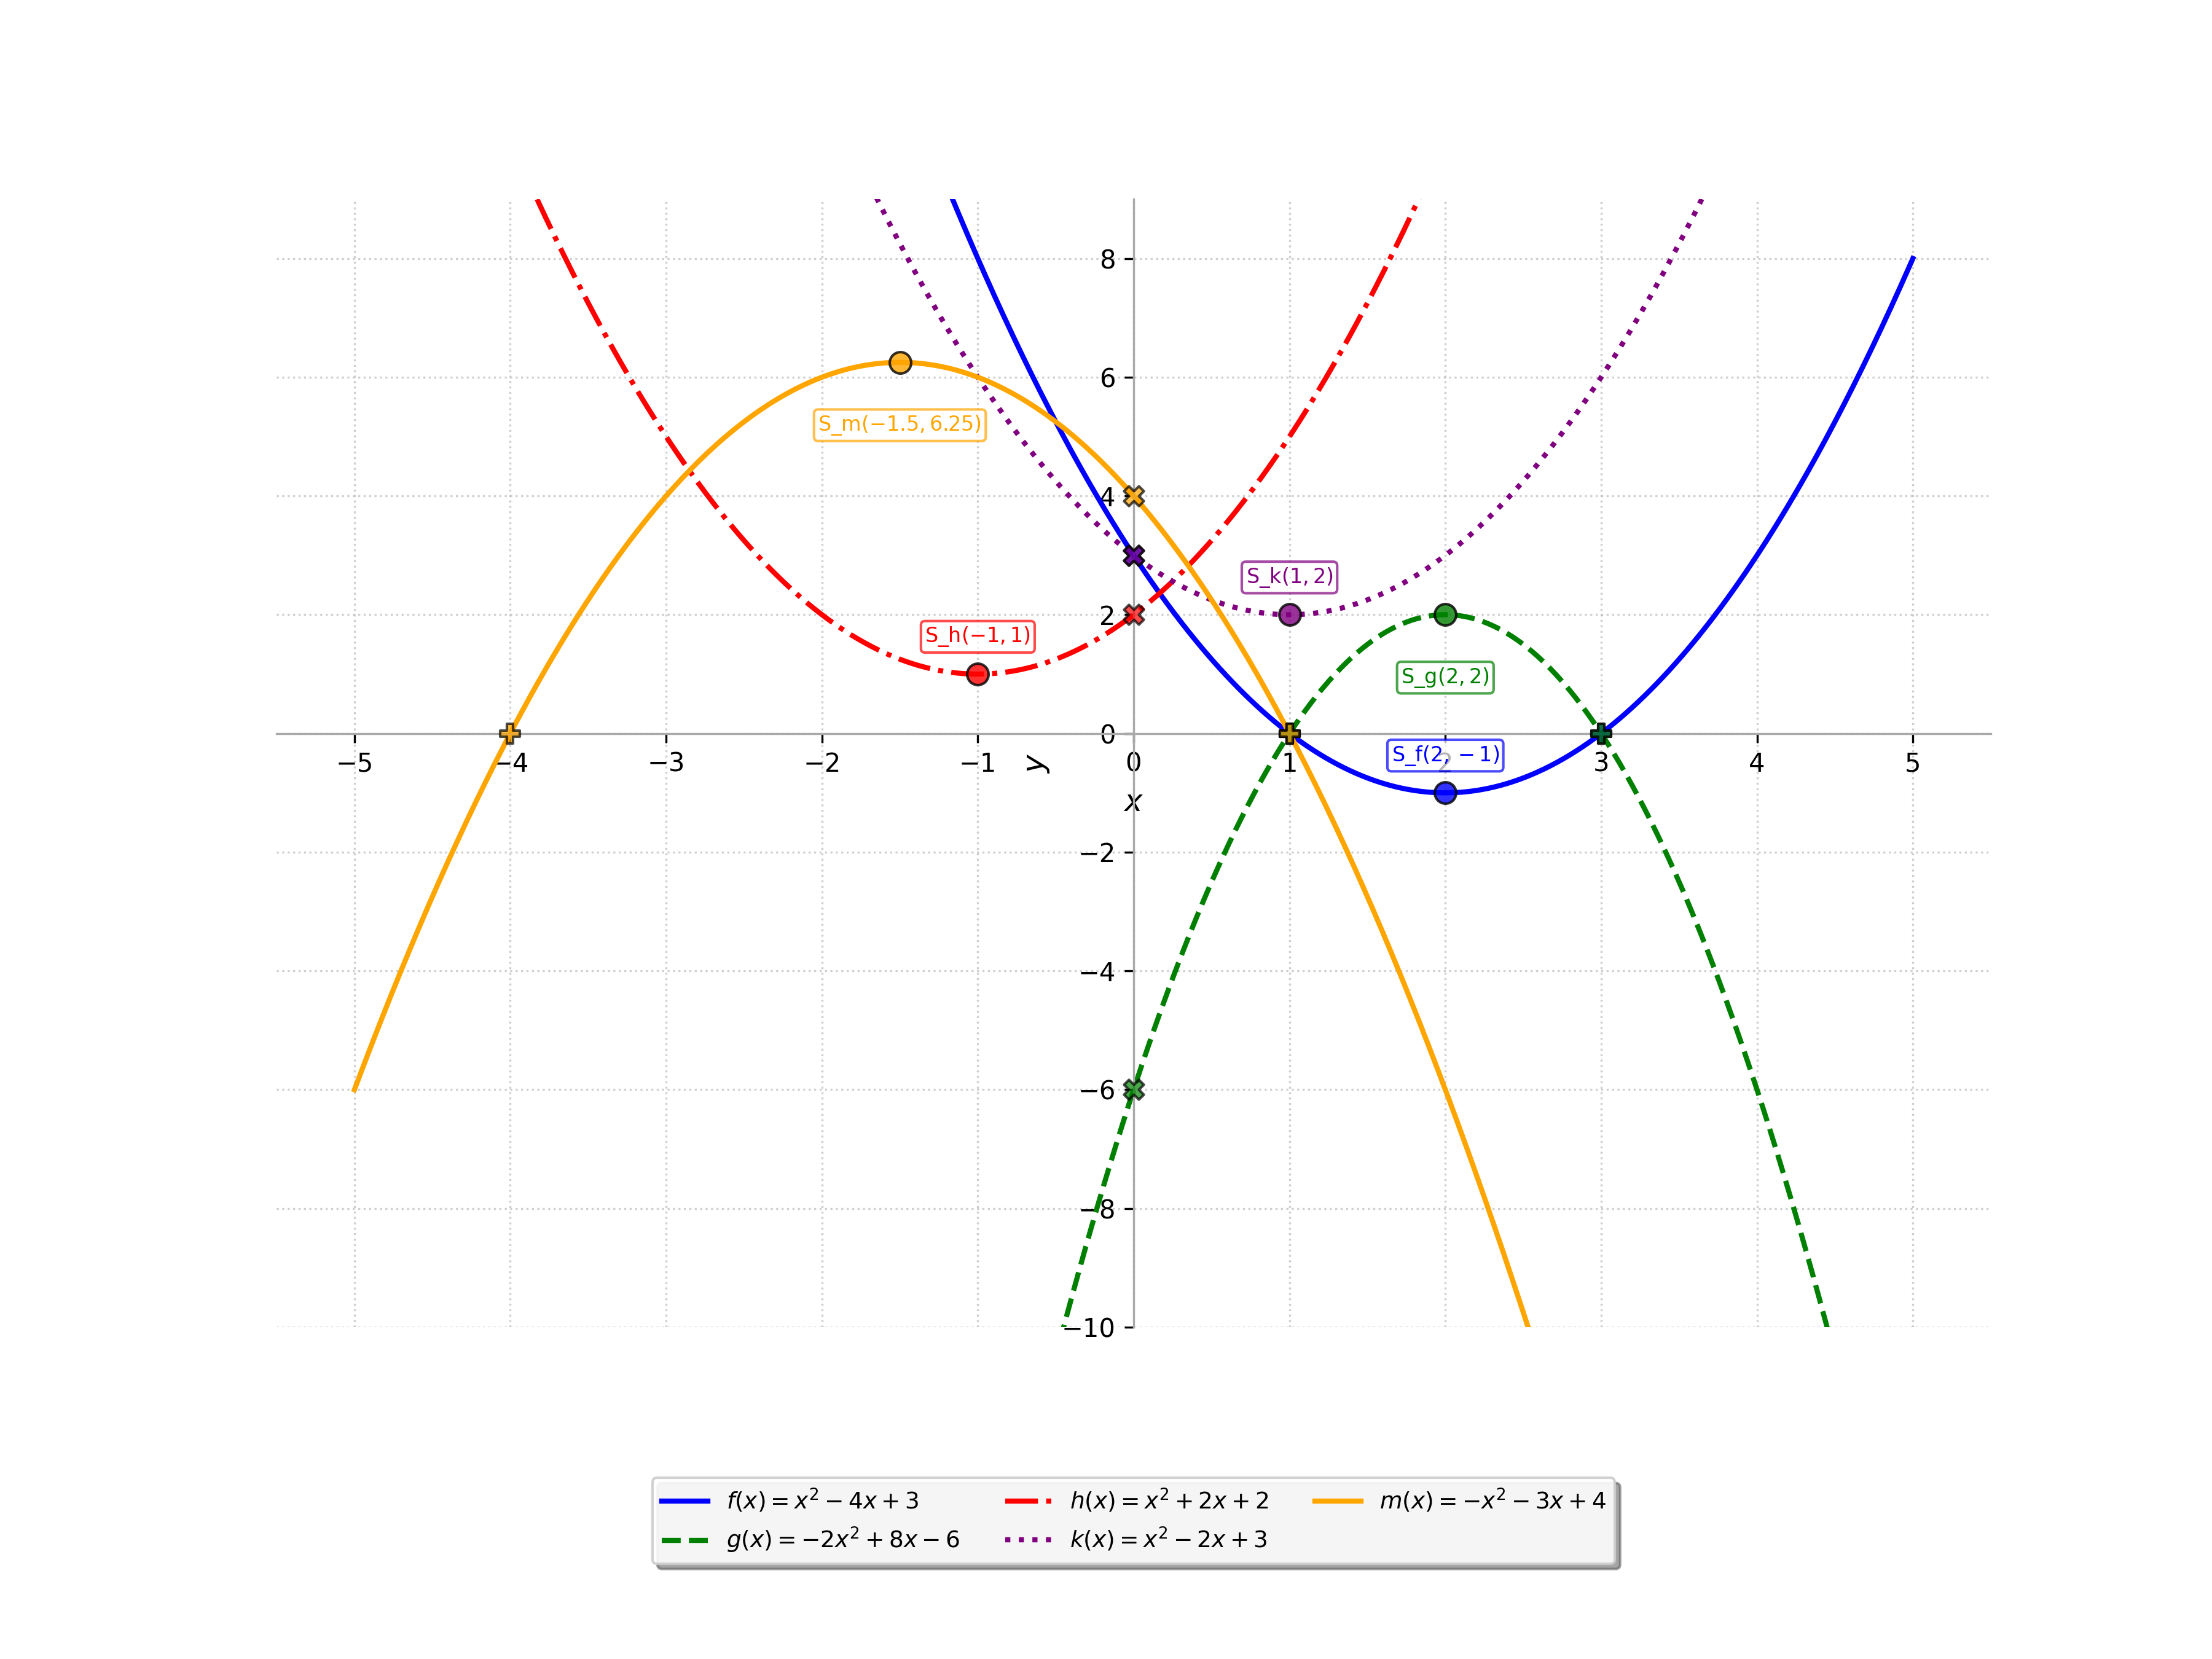
\includegraphics[width=0.8\textwidth]{grafiken/kurvendiskussion_kombi_graph.png}
% --- Beschreibung der Grafik ---
% Die Grafik zeigt ein kartesisches Koordinatensystem.
% Die x-Achse ist beschriftet und skaliert, um die relevanten x-Werte aller Parabeln darzustellen (z.B. von -5 bis 5).
% Die y-Achse ist beschriftet und skaliert, um die relevanten y-Werte aller Parabeln darzustellen (z.B. von -7 bis 8).
% Fünf Parabeln sind eingezeichnet und idealerweise durch unterschiedliche Farben oder Linienstile sowie Beschriftungen (f(x), g(x), h(x), k(x), m(x)) gekennzeichnet:
% 1. f(x) = x^2 - 4x + 3: S(2|-1), N(1|0), N(3|0), Py(0|3), nach oben offen.
% 2. g(x) = -2x^2 + 8x - 6: S(2|2), N(1|0), N(3|0), Py(0|-6), nach unten offen, schmaler.
% 3. h(x) = x^2 + 2x + 2: S(-1|1), keine Nullstellen, Py(0|2), nach oben offen.
% 4. k(x) = x^2 - 2x + 3: S(1|2), keine Nullstellen, Py(0|3), nach oben offen.
% 5. m(x) = -x^2 - 3x + 4: S(-1.5|6.25), N(-4|0), N(1|0), Py(0|4), nach unten offen.
% Wichtige Punkte (Scheitelpunkte, Achsenschnittpunkte) sollten für jede Parabel durch die Zeichnung plausibel erscheinen.
\captionof{figure}{Graphen der Funktionen $f(x)$, $g(x)$, $h(x)$, $k(x)$ und $m(x)$ im Vergleich.}
\label{fig:kurvendiskussion_kombi}
\end{center}

\end{loesungsumgebung}



\begin{aufgabenumgebung}[Brückenbogen]{Der Brückenbogen – eine klassische Anwendung}
Ein parabelförmiger Brückenbogen wird durch eine quadratische Funktion $f(x)$ beschrieben. Der Ursprung des Koordinatensystems $(0|0)$ liegt direkt unter der Mitte des Bogens auf Wasserniveau (x-Achse).
Der Bogen beginnt und endet auf Wasserniveau bei $x=-20\,$m und $x=20\,$m. In der Mitte (also bei $x=0$) ist der Bogen $8\,$m hoch.
\begin{enumerate}
    \item \textbf{Informationen sammeln:} Welche drei Punkte des Graphen der Funktion $f(x)$ sind dir damit bekannt? Notiere ihre Koordinaten.
    \item \textbf{Funktionsgleichung bestimmen:}
        \begin{itemize}
            \item Da der Scheitelpunkt offensichtlich auf der y-Achse liegt (genau in der Mitte bei $x=0$), welche Form hat die quadratische Funktion dann? (Tipp: Welcher Koeffizient ist Null?)
            \item Nutze den Punkt $(0|8)$, um den Koeffizienten $c$ zu bestimmen.
            \item Nutze einen der anderen Punkte (z.B. $(20|0)$), um den Koeffizienten $a$ zu bestimmen.
            \item Schreibe die vollständige Funktionsgleichung $f(x)$ des Brückenbogens auf.
        \end{itemize}
    \item \textbf{Anwendung der Funktion:} Wie hoch ist der Brückenbogen an der Stelle $x=10\,$m vom Mittelpunkt aus gemessen?
    \item \textbf{Skizze:} Erstelle eine Skizze des Brückenbogens im Koordinatensystem.
\end{enumerate}
\end{aufgabenumgebung}


\begin{loesungsumgebung}[loes:Brueckenbogen]{Der Brückenbogen – eine klassische Anwendung}

\begin{enumerate}[label=(\alph*)]
    \item \textbf{Informationen sammeln:}
    Aus der Problembeschreibung können wir die folgenden drei Punkte des Graphen der Funktion $f(x)$ entnehmen:
    \begin{itemize}
        \item Der Bogen beginnt auf Wasserniveau bei $x=-20\,$m: $N_1(-20|0)$.
        \item Der Bogen endet auf Wasserniveau bei $x=20\,$m: $N_2(20|0)$.
        \item In der Mitte (bei $x=0$) ist der Bogen $8\,$m hoch: Dies ist der Scheitelpunkt $S(0|8)$.
    \end{itemize}

    \item \textbf{Funktionsgleichung bestimmen:}
    \begin{itemize}
        \item Da der Scheitelpunkt bei $x=0$ auf der y-Achse liegt, ist die Parabel achsensymmetrisch zur y-Achse. Das bedeutet, dass der Koeffizient $b$ in der allgemeinen quadratischen Funktionsgleichung $f(x) = ax^2+bx+c$ Null ist ($b=0$). Die Funktion hat also die Form $f(x) = ax^2+c$.
        \item Der Scheitelpunkt einer solchen Parabel ist $S(0|c)$. Da wir wissen, dass der Scheitelpunkt $S(0|8)$ ist, können wir direkt ablesen, dass $c=8$.
        Die Funktion lautet somit bisher: $f(x) = ax^2+8$.
        \item Um den Koeffizienten $a$ zu bestimmen, setzen wir die Koordinaten eines der anderen bekannten Punkte (z.B. $N_2(20|0)$) in die Funktionsgleichung $f(x) = ax^2+8$ ein:
        $f(20) = 0 \Rightarrow a(20)^2+8 = 0$.
        $$a(400)+8 = 0$$
        Umformungsschritte:
        $$
        \begin{array}{r c l c l}
        \umformung{400a + 8}{0}{-}{8}
        \umformung{400a}{-8}{\div}{400}
        \umformungend{a}{-\frac{8}{400}}
        \end{array}
        $$
        $a = -\frac{8}{400} = -\frac{1}{50} = -0.02$.
        \item Die vollständige Funktionsgleichung des Brückenbogens lautet:
        $$f(x) = -0.02x^2 + 8$$
    \end{itemize}

    \item \textbf{Anwendung der Funktion:}
    Um die Höhe des Brückenbogens an der Stelle $x=10\,$m vom Mittelpunkt aus zu bestimmen, setzen wir $x=10$ in die Funktionsgleichung ein:
    $$f(10) = -0.02(10)^2 + 8$$
    $$f(10) = -0.02(100) + 8$$
    $$f(10) = -2 + 8$$
    $$f(10) = 6$$
    An der Stelle $x=10\,$m ist der Brückenbogen $6\,$m hoch.

    \item \textbf{Skizze:}
    Eine Skizze des Brückenbogens $f(x) = -0.02x^2 + 8$ würde Folgendes zeigen:
    \begin{itemize}
        \item Eine nach unten geöffnete Parabel (da $a=-0.02 < 0$).
        \item Der Scheitelpunkt (höchster Punkt) liegt bei $S(0|8)$.
        \item Die Nullstellen (Schnittpunkte mit der x-Achse, dem Wasserniveau) liegen bei $N_1(-20|0)$ und $N_2(20|0)$.
        \item Der Punkt $P(10|6)$ (und symmetrisch $P'(-10|6)$) liegt auf dem Bogen.
        \item Die x-Achse repräsentiert das Wasserniveau, die y-Achse die Höhe. Der Bogen verläuft nur für $x \in [-20, 20]$ im relevanten Bereich oberhalb oder auf dem Wasserniveau.
    \end{itemize}
    Die im Aufgabenstellungstext bereits eingefügte Abbildung gibt eine allgemeine Vorstellung eines solchen Brückenbogens. 

\end{enumerate}
\end{loesungsumgebung}

\begin{aufgabenumgebung}{Flugbahn eines Balls}
Ein Ball wird schräg nach oben geworfen. Seine Flughöhe $h(x)$ in Metern über dem Boden kann in Abhängigkeit von der horizontalen Entfernung $x$ (in Metern vom Abwurfpunkt) durch die Funktion
\[ h(x) = -0.1x^2 + 1.2x + 1.6 \]
beschrieben werden (für $x \ge 0$ und solange $h(x) \ge 0$).
\begin{enumerate}
    \item \textbf{Abwurfhöhe:} Aus welcher Höhe wurde der Ball abgeworfen? (Tipp: Das ist die Höhe an der Stelle $x=0$.)
    \item \textbf{Maximale Flughöhe:} Berechne die maximale Flughöhe des Balls. (Tipp: Das ist die y-Koordinate des Scheitelpunkts.)
    \item \textbf{Horizontale Entfernung bei max. Höhe:} Bei welcher horizontalen Entfernung vom Abwurfpunkt erreicht der Ball seine maximale Höhe? (Tipp: Das ist die x-Koordinate des Scheitelpunkts.)
    \item \textbf{Wurfweite:} Bei welcher horizontalen Entfernung trifft der Ball wieder auf dem Boden auf? (Tipp: Gesucht ist die positive Nullstelle der Funktion, da $h(x)=0$ bedeutet, dass der Ball auf dem Boden ist.)
    \item \textbf{Skizze:} Skizziere die Flugbahn des Balls (den Graphen von $h(x)$ im relevanten Bereich). Markiere Abwurfpunkt, höchsten Punkt und Auftreffpunkt.
\end{enumerate}
\end{aufgabenumgebung}

\begin{loesungsumgebung}[loes:flugbahn-ball]{Flugbahn eines Balls}
Die Flughöhe des Balls wird durch die quadratische Funktion $h(x) = -0.1x^2 + 1.2x + 1.6$ beschrieben, wobei $a=-0.1$, $b=1.2$ und $c=1.6$.

\begin{enumerate}[label=(\alph*)]
    \item \textbf{Abwurfhöhe:}
    Die Abwurfhöhe ist die Höhe an der Stelle $x=0$ (horizontale Entfernung vom Abwurfpunkt ist Null).
    $$ h(0) = -0.1(0)^2 + 1.2(0) + 1.6 = 0 + 0 + 1.6 = 1.6 $$
    Der Ball wurde aus einer Höhe von \textbf{1,6 Metern} abgeworfen.

    \item \textbf{Maximale Flughöhe:}
    Die maximale Flughöhe ist die y-Koordinate des Scheitelpunkts ($y_S$) der Parabel. Zuerst berechnen wir die x-Koordinate des Scheitelpunkts $x_S = -\frac{b}{2a}$.
    $$ x_S = -\frac{1.2}{2 \cdot (-0.1)} = -\frac{1.2}{-0.2} = \frac{1.2}{0.2} = 6 $$
    Nun setzen wir $x_S=6$ in die Funktion $h(x)$ ein, um $y_S$ zu erhalten:
    $$ y_S = h(6) = -0.1(6)^2 + 1.2(6) + 1.6 $$
    $$ y_S = -0.1(36) + 7.2 + 1.6 $$
    $$ y_S = -3.6 + 7.2 + 1.6 $$
    $$ y_S = 3.6 + 1.6 = 5.2 $$
    Die maximale Flughöhe des Balls beträgt \textbf{5,2 Meter}.

    \item \textbf{Horizontale Entfernung bei max. Höhe:}
    Dies ist die x-Koordinate des Scheitelpunkts, $x_S$, die wir in Teil (b) berechnet haben.
    Der Ball erreicht seine maximale Höhe bei einer horizontalen Entfernung von \textbf{6 Metern} vom Abwurfpunkt.

    \item \textbf{Wurfweite:}
    Die Wurfweite ist die horizontale Entfernung, bei der der Ball wieder auf dem Boden auftrifft, d.h. $h(x)=0$. Wir suchen die positive Nullstelle der Funktion.
    $$ -0.1x^2 + 1.2x + 1.6 = 0 $$
    Wir verwenden die Mitternachtsformel (ABC-Formel) $x_{1,2} = \frac{-b \pm \sqrt{b^2-4ac}}{2a}$.
    Die Diskriminante $D$ ist:
    $$ D = b^2 - 4ac = (1.2)^2 - 4(-0.1)(1.6) = 1.44 - (-0.64) = 1.44 + 0.64 = 2.08 $$
    Die Nullstellen sind:
    $$ x_{1,2} = \frac{-1.2 \pm \sqrt{2.08}}{2(-0.1)} = \frac{-1.2 \pm \sqrt{2.08}}{-0.2} $$
    Wir können $\sqrt{2.08}$ auch als $\sqrt{\frac{208}{100}} = \frac{\sqrt{16 \cdot 13}}{10} = \frac{4\sqrt{13}}{10} = \frac{2\sqrt{13}}{5}$ schreiben.
    $$ x_{1,2} = \frac{-1.2 \pm \frac{2\sqrt{13}}{5}}{-0.2} = \frac{-\frac{6}{5} \pm \frac{2\sqrt{13}}{5}}{-\frac{1}{5}} $$
    Multiplikation von Zähler und Nenner mit $-5$:
    $$ x_{1,2} = 6 \mp 2\sqrt{13} $$
    Die beiden Nullstellen sind:
    $$ x_1 = 6 - 2\sqrt{13} \approx 6 - 2 \cdot 3.60555 \approx 6 - 7.2111 \approx -1.2111 $$
    $$ x_2 = 6 + 2\sqrt{13} \approx 6 + 2 \cdot 3.60555 \approx 6 + 7.2111 \approx 13.2111 $$
    Da die horizontale Entfernung $x$ nicht negativ sein kann ($x \ge 0$), ist die Wurfweite die positive Nullstelle $x_2$.
    Der Ball trifft bei einer horizontalen Entfernung von $6 + 2\sqrt{13}$ Metern (ca. \textbf{13,21 Metern}) wieder auf dem Boden auf.
\end{enumerate}

\end{loesungsumgebung}


\begin{aufgabenumgebung}[labelA:QuadratischeAnw]{Weitere Anwendungs- und Verständnisaufgaben}
\begin{enumerate}
    \item \textbf{Rechteck mit maximaler Fläche:} Ein Bauer hat 40 Meter Zaun und möchte damit ein rechteckiges Feld an einer langen, geraden Mauer abgrenzen. Die Seite an der Mauer braucht keinen Zaun. Welche Abmessungen (Länge und Breite) sollte das Feld haben, damit seine Fläche maximal wird?
        \begin{itemize}
            \item Sei $x$ die Länge der Seite, die senkrecht zur Mauer steht. Drücke die andere Zaunseite (parallel zur Mauer) ebenfalls durch $x$ aus (bedenke die 40m Gesamtzaunlänge).
            \item Stelle eine Funktion $A(x)$ für die Fläche des Rechtecks in Abhängigkeit von $x$ auf.
            \item Bestimme den Scheitelpunkt dieser quadratischen Funktion $A(x)$. Was bedeuten die Koordinaten des Scheitelpunkts für das Problem?
            \item Gib die optimalen Abmessungen und die maximale Fläche an.
        \end{itemize}
    \item \textbf{Funktion aus Scheitelpunkt und Punkt finden:} Eine Parabel hat ihren Scheitelpunkt bei $S(2|-1)$ und geht durch den Punkt $P(4|7)$. Bestimme ihre Funktionsgleichung. (Tipp: Setze den Scheitelpunkt in die Scheitelpunktform $f(x)=a(x-x_S)^2+y_S$ ein. Setze dann die Koordinaten von $P$ ein, um $a$ zu berechnen.)
    \item \textbf{Funktion aus Nullstellen und Punkt finden:} Eine Parabel schneidet die x-Achse bei $x_1=-1$ und $x_2=3$. Außerdem geht sie durch den Punkt $P(1|-4)$. Bestimme ihre Funktionsgleichung. (Tipp: Nutze die faktorisierte Form einer quadratischen Funktion: $f(x)=a(x-x_1)(x-x_2)$, die wir im Merksatz \ref{merksatz:faktorisierte_form} kennengelernt haben. Setze die Nullstellen ein und dann den Punkt $P$, um $a$ zu berechnen.)
    \item \textbf{Parameter untersuchen:} Gegeben ist die Funktionenschar $f_k(x) = x^2 - 2kx + 4$ mit dem Parameter $k \in \mathbb{R}$.
        \begin{itemize}
            \item Bestimme die Koordinaten des Scheitelpunkts in Abhängigkeit von $k$.
            \item Für welche Werte von $k$ hat die Funktion genau eine Nullstelle? Keine Nullstellen? Zwei Nullstellen? (Tipp: Untersuche die Diskriminante $D$ in Abhängigkeit von $k$.)
            \item Auf welcher Kurve liegen alle Scheitelpunkte der Schar $f_k(x)$? (Tipp: Drücke $y_S$ durch $x_S$ aus. Diese Kurve nennt man auch \textit{Ortskurve} der Scheitelpunkte.)
        \end{itemize}
\end{enumerate}
\end{aufgabenumgebung}


\begin{loesungsumgebung}[loes:QuadratischeAnw]{Weitere Anwendungs- und Verständnisaufgaben}

\begin{enumerate}
    \item \textbf{Rechteck mit maximaler Fläche:}
    Ein Bauer hat 40 Meter Zaun für ein rechteckiges Feld an einer Mauer.
    \begin{itemize}
        \item \textbf{Seitenlängen ausdrücken:} \\
        Sei $x$ die Länge der Seite, die senkrecht zur Mauer steht (in Metern). Es gibt zwei solcher Seiten. Der Zaunverbrauch für diese beiden Seiten ist $2x$.
        Die Länge der Seite parallel zur Mauer ist dann der verbleibende Zaun: $L_{parallel} = 40 - 2x$ (in Metern).

        \item \textbf{Flächenfunktion $A(x)$ aufstellen:} \\
        Die Fläche $A$ des Rechtecks ist $A = \text{Breite} \cdot \text{Länge}$. Hier:
        $A(x) = x \cdot (40 - 2x) = 40x - 2x^2$.
        In Standardform: $A(x) = -2x^2 + 40x$.

        \item \textbf{Scheitelpunkt dieser quadratischen Funktion $A(x)$ bestimmen:} \\
        Die Funktion $A(x) = -2x^2 + 40x$ hat die Koeffizienten $a=-2$, $b=40$, $c=0$.
        Die x-Koordinate des Scheitelpunkts ist $x_S = -\frac{b}{2a}$:
        $$ x_S = -\frac{40}{2 \cdot (-2)} = -\frac{40}{-4} = 10 $$
        Die y-Koordinate des Scheitelpunkts (maximale Fläche) ist $y_S = A(x_S) = A(10)$:
        $$ A(10) = -2(10)^2 + 40(10) = -2(100) + 400 = -200 + 400 = 200 $$
        Der Scheitelpunkt ist $S(10|200)$.
        \textbf{Bedeutung der Koordinaten:} $x_S=10\,$m ist die Länge der senkrechten Seite, bei der die Fläche maximal wird. $y_S=200\,$m$^2$ ist diese maximale Fläche. Da $a=-2 < 0$, handelt es sich tatsächlich um ein Maximum.

        \item \textbf{Optimale Abmessungen und maximale Fläche angeben:}
        \begin{itemize}
            \item Länge der Seiten senkrecht zur Mauer: $x = 10\,$m.
            \item Länge der Seite parallel zur Mauer: $40 - 2x = 40 - 2(10) = 20\,$m.
            \item Maximale Fläche: $A_{max} = 200\,$m$^2$.
        \end{itemize}
        Die optimalen Abmessungen sind $10\,$m (Tiefe von der Mauer weg) und $20\,$m (Länge entlang der Mauer).
    \end{itemize}

    \item \textbf{Funktion aus Scheitelpunkt und Punkt finden:}
    Eine Parabel hat ihren Scheitelpunkt bei $S(2|-1)$ und geht durch den Punkt $P(4|7)$.
    Wir nutzen die Scheitelpunktform $f(x) = a(x-x_S)^2 + y_S$.
    Mit $x_S=2$ und $y_S=-1$:
    $$ f(x) = a(x-2)^2 - 1 $$
    Nun setzen wir den Punkt $P(4|7)$ ein ($x=4, f(x)=7$), um $a$ zu bestimmen:
    $$ 7 = a(4-2)^2 - 1 $$
    $$ 7 = a(2)^2 - 1 $$
    $$ 7 = 4a - 1 $$
    Umformungsschritte:
    $$
    \begin{array}{r c l c l}
    \umformung{4a - 1}{7}{+}{1}
    \umformung{4a}{8}{\div}{4}
    \umformungend{a}{2}
    \end{array}
    $$
    Also ist $a=2$. Die Funktionsgleichung lautet:
    $$ f(x) = 2(x-2)^2 - 1 $$
    (Ausmultipliziert: $f(x) = 2(x^2-4x+4)-1 = 2x^2-8x+8-1 = 2x^2-8x+7$).

    \item \textbf{Funktion aus Nullstellen und Punkt finden:}
    Eine Parabel schneidet die x-Achse bei $x_1=-1$ und $x_2=3$ und geht durch $P(1|-4)$.
    Wir nutzen die faktorisierte Form $f(x) = a(x-x_1)(x-x_2)$.
    Mit $x_1=-1$ und $x_2=3$:
    $$ f(x) = a(x-(-1))(x-3) = a(x+1)(x-3) $$
    Nun setzen wir den Punkt $P(1|-4)$ ein ($x=1, f(x)=-4$), um $a$ zu bestimmen:
    $$ -4 = a(1+1)(1-3) $$
    $$ -4 = a(2)(-2) $$
    $$ -4 = -4a $$
    Umformungsschritte:
    $$
    \begin{array}{r c l c l}
    \umformung{-4a}{-4}{\div}{(-4)}
    \umformungend{a}{1}
    \end{array}
    $$
    Also ist $a=1$. Die Funktionsgleichung lautet:
    $$ f(x) = 1(x+1)(x-3) = (x+1)(x-3) $$
    (Ausmultipliziert: $f(x) = x^2-3x+x-3 = x^2-2x-3$).

    \item \textbf{Parameter untersuchen:} Gegeben ist die Funktionenschar $f_k(x) = x^2 - 2kx + 4$.
    Koeffizienten: $A=1, B=-2k, C=4$ (Großbuchstaben zur Unterscheidung vom Parameter $k$).
    \begin{itemize}
        \item \textbf{Koordinaten des Scheitelpunkts in Abhängigkeit von $k$:} \\
        $x_S(k) = -\frac{B}{2A} = -\frac{-2k}{2(1)} = \frac{2k}{2} = k$. \\
        $y_S(k) = f_k(x_S(k)) = f_k(k) = (k)^2 - 2k(k) + 4 = k^2 - 2k^2 + 4 = -k^2 + 4$. \\
        Der Scheitelpunkt ist $S_k(k | -k^2+4)$.

        \item \textbf{Anzahl der Nullstellen in Abhängigkeit von $k$:} \\
        Wir untersuchen die Diskriminante $D = B^2 - 4AC$:
        $D = (-2k)^2 - 4(1)(4) = 4k^2 - 16$.
        \begin{itemize}
            \item \textit{Genau eine Nullstelle:} $D=0$.
            $4k^2 - 16 = 0$
            $$
            \begin{array}{r c l c l}
            \umformung{4k^2 - 16}{0}{+}{16}
            \umformung{4k^2}{16}{\div}{4}
            \umformungend{k^2}{4}
            \end{array}
            $$
            Aus $k^2=4$ folgt $k = \pm\sqrt{4}$, also $k_1=2$ und $k_2=-2$.
            Für $k=2$ oder $k=-2$ gibt es genau eine Nullstelle.
            \item \textit{Zwei verschiedene Nullstellen:} $D>0$.
            $4k^2 - 16 > 0 \implies 4k^2 > 16 \implies k^2 > 4$.
            Dies ist erfüllt für $k < -2$ oder $k > 2$. (Intervall: $(-\infty, -2) \cup (2, \infty)$).
            \item \textit{Keine Nullstellen:} $D<0$.
            $4k^2 - 16 < 0 \implies 4k^2 < 16 \implies k^2 < 4$.
            Dies ist erfüllt für $-2 < k < 2$. (Intervall: $(-2, 2)$).
        \end{itemize}

        \item \textbf{Ortskurve der Scheitelpunkte:} \\
        Wir haben die Koordinaten des Scheitelpunkts in Abhängigkeit von $k$:
        $x_S = k$
        $y_S = -k^2 + 4$
        Um $y_S$ durch $x_S$ auszudrücken, setzen wir $k=x_S$ in die Gleichung für $y_S$ ein:
        $$ y_S = -(x_S)^2 + 4 $$
        Die Ortskurve der Scheitelpunkte ist eine Parabel mit der Gleichung $y = -x^2 + 4$.
    \end{itemize}
\end{enumerate}

\end{loesungsumgebung}

\begin{aufgabenumgebung}{Checkliste: Parabeln verstehen – Mehr als nur Formeln}
Diese Aufgabe soll dir helfen, dein qualitatives Verständnis für quadratische Funktionen und ihre Graphen (Parabeln) zu vertiefen. Oft kann man schon viel über eine Parabel aussagen, ohne gleich jede Formel parat haben zu müssen! Nutze für deine Argumentationen auch immer kleine Skizzen.

\begin{enumerate}[label=\textbf{Teil \arabic*:}]
    \item \textbf{Argumentieren mit Nullstellen und dem Öffnungsfaktor $a$} \\
    Stell dir vor, du kennst von einer quadratischen Funktion $f(x)=ax^2+bx+c$ die Nullstellen (also die $x$-Werte, an denen $f(x)=0$ ist) und das Vorzeichen des Parameters $a$.

    \begin{enumerate}[label=(\alph*)]
        \item Eine Parabel hat die Nullstellen $x_1 = -1$ und $x_2 = 5$. Der Öffnungsfaktor ist $a > 0$.
        \begin{itemize}
            \item Skizziere diese Parabel grob. Ist sie nach oben oder nach unten geöffnet?
            \item In welchen $x$-Bereichen (Intervallen) verlaufen die Funktionswerte $f(x)$ oberhalb der x-Achse (sind also positiv)? In welchen Bereichen verlaufen sie unterhalb (sind also negativ)? Begründe mit deiner Skizze.
            \item Ohne den Scheitelpunkt genau zu berechnen: Was kannst du über die Lage seiner x-Koordinate $x_S$ sagen? (Tipp: Symmetrie!)
        \end{itemize}
        \item Betrachte nun eine andere Parabel mit denselben Nullstellen $x_1 = -1$ und $x_2 = 5$, aber diesmal mit einem Öffnungsfaktor $a < 0$.
        \begin{itemize}
            \item Skizziere auch diesen Fall. Wie ändern sich die Antworten auf die Fragen aus (a) bezüglich Öffnung und Vorzeichen der Funktionswerte?
        \end{itemize}
    \end{enumerate}

    \item \textbf{Argumentieren mit dem y-Achsenabschnitt $c$ und dem Öffnungsfaktor $a$ (Nullstellen sind unbekannt)} \\
    Stell dir vor, du kennst von einer quadratischen Funktion $f(x)=ax^2+bx+c$ nur den y-Achsenabschnitt $c$ (also den Wert $f(0)$) und das Vorzeichen des Öffnungsfaktors $a$.

    \begin{enumerate}[label=(\alph*)]
        \item Eine Parabel ist nach oben geöffnet ($a > 0$) und schneidet die y-Achse bei $c = -2$.
        \begin{itemize}
            \item Skizziere zwei \textit{mögliche} Verläufe für diese Parabel.
            \item Muss diese Parabel zwangsläufig Nullstellen besitzen? Begründe deine Antwort (denke an die Lage des Scheitelpunkts).
            \item Was kannst du über den y-Wert des Scheitelpunkts $y_S$ im Vergleich zum y-Achsenabschnitt $c$ sagen? Ist $y_S \leq c$, $y_S \geq c$ oder kann das variieren? Begründe.
        \end{itemize}
        \item Eine Parabel ist nach unten geöffnet ($a < 0$) und schneidet die y-Achse bei $c = 3$.
        \begin{itemize}
            \item Skizziere auch hier zwei \textit{mögliche} Verläufe.
            \item Kannst du mit Sicherheit sagen, ob diese Parabel Nullstellen hat? Oder ob sie keine hat? Oder ist beides möglich? Erkläre deine Überlegungen.
        \end{itemize}
        \item Eine Parabel ist nach oben geöffnet ($a > 0$) und ihr y-Achsenabschnitt $c$ ist ebenfalls positiv ($c > 0$, z.B. $c=4$).
        \begin{itemize}
            \item Beschreibe und skizziere die drei Möglichkeiten für die Anzahl der Nullstellen (keine, eine, zwei).
            \item Welche Bedingung muss für den Scheitelpunkt (insbesondere dessen y-Koordinate $y_S$) erfüllt sein, damit die Parabel in diesem Fall
            \begin{itemize}
                \item keine Nullstellen hat?
                \item genau eine Nullstelle hat?
                \item zwei Nullstellen hat?
            \end{itemize}
        \end{itemize}
    \end{enumerate}
\end{enumerate}
Versuche, deine Antworten immer auch mit kleinen, beschrifteten Skizzen zu untermauern!
\end{aufgabenumgebung}



\begin{loesungsumgebung}[loes:parabeln-verstehen-qualitativ-konsolidiert]{Checkliste: Parabeln verstehen – Mehr als nur Formeln}

\begin{enumerate}[label=\textbf{Teil \arabic*:}]
    \item \textbf{Argumentieren mit Nullstellen und dem Öffnungsfaktor $a$} \\
    Gegeben ist eine quadratische Funktion $f(x)=ax^2+bx+c$.
    Die Skizzen zu diesem Teil sind in Abbildung \ref{fig:parabeln_teil1_vergleich_a} zusammengefasst.

    \begin{enumerate}[label=(\alph*)]
        \item Eine Parabel hat die Nullstellen $x_1 = -1$ und $x_2 = 5$. Der Öffnungsfaktor ist $a > 0$.
        \begin{itemize}
            \item \textbf{Skizze und Öffnung:} \\
            Da $a > 0$, ist die Parabel \textbf{nach oben geöffnet}. Sie schneidet die x-Achse an den Stellen $x=-1$ und $x=5$. (Siehe Abb. \ref{fig:parabeln_teil1_vergleich_a}, Fall 1)

            \item \textbf{Vorzeichen der Funktionswerte $f(x)$:}
            \begin{itemize}
                \item $f(x)$ ist \textbf{positiv} ($f(x)>0$) für $x < -1$ oder $x > 5$. (Bereiche außerhalb der Nullstellen).
                \item $f(x)$ ist \textbf{negativ} ($f(x)<0$) für $-1 < x < 5$. (Bereich zwischen den Nullstellen).
            \end{itemize}
            \textit{Begründung:} Die nach oben geöffnete Parabel kommt von $+\infty$, fällt bis zu ihrem Scheitelpunkt (zwischen den Nullstellen, unterhalb der x-Achse) und steigt dann wieder zu $+\infty$.

            \item \textbf{Lage der x-Koordinate des Scheitelpunkts $x_S$:} \\
            Aufgrund der Symmetrie liegt $x_S$ genau in der Mitte zwischen den Nullstellen:
            $ x_S = \frac{-1 + 5}{2} = 2 $.
        \end{itemize}

        \item Eine andere Parabel mit denselben Nullstellen $x_1 = -1$ und $x_2 = 5$, aber mit $a < 0$.
        \begin{itemize}
            \item \textbf{Skizze und Änderungen:} \\
            Da $a < 0$, ist diese Parabel \textbf{nach unten geöffnet}. Sie schneidet die x-Achse ebenfalls bei $x=-1$ und $x=5$. (Siehe Abb. \ref{fig:parabeln_teil1_vergleich_a}, Fall 2)
            \textbf{Änderungen im Vergleich zu (a):}
            \begin{itemize}
                \item \textbf{Öffnung:} Die Parabel ist nach unten geöffnet.
                \item \textbf{Vorzeichen der Funktionswerte $f(x)$:} Das Verhalten kehrt sich um.
                    \begin{itemize}
                        \item $f(x)$ ist \textbf{positiv} für $-1 < x < 5$.
                        \item $f(x)$ ist \textbf{negativ} für $x < -1$ oder $x > 5$.
                    \end{itemize}
                \item Die x-Koordinate des Scheitelpunkts $x_S=2$ bleibt gleich. Der Scheitelpunkt ist nun ein Hochpunkt (oberhalb der x-Achse).
            \end{itemize}
        \end{itemize}
    \end{enumerate}
    \begin{center}
    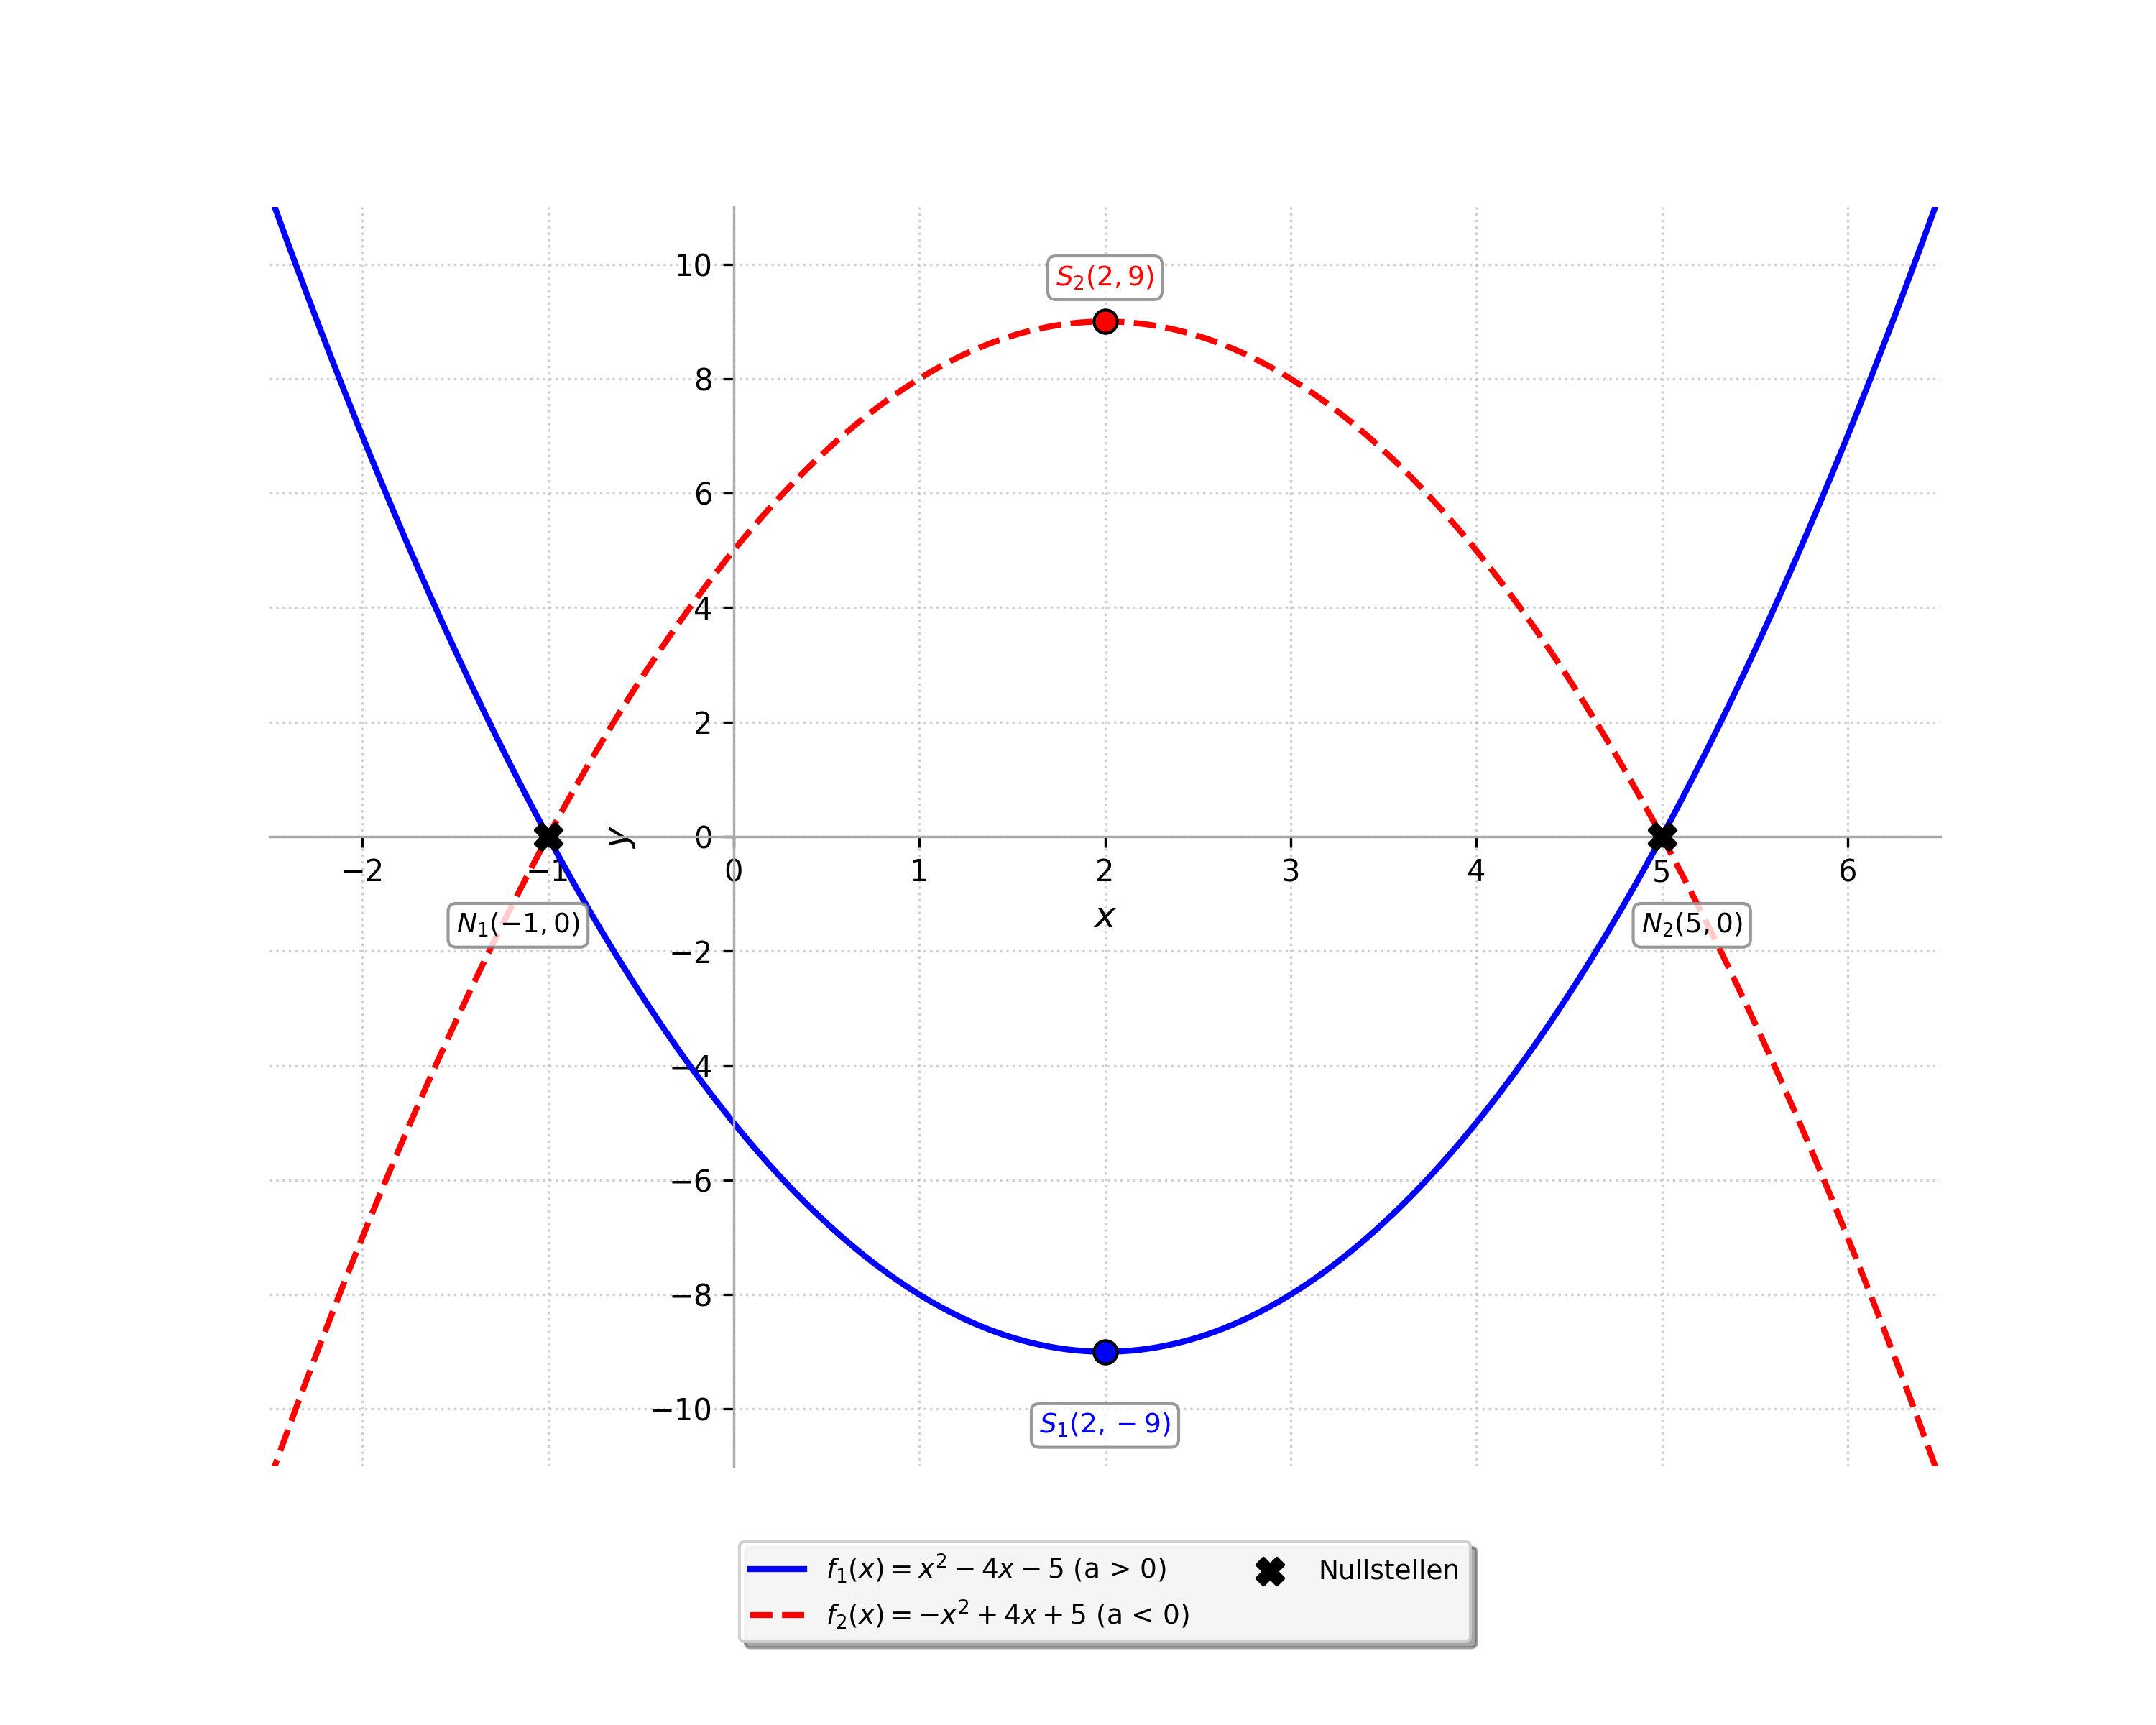
\includegraphics[width=0.8\textwidth]{grafiken/parabeln_teil1_vergleich_a.png}
    % --- Beschreibung der zusammengefassten Skizze für Teil 1 ---
    % Die Abbildung zeigt ein einzelnes Koordinatensystem.
    % Darin sind ZWEI Parabeln skizziert:
    % 1. Fall 1 (aus 1a): Nach oben geöffnete Parabel (a > 0), schneidet die x-Achse bei x = -1 und x = 5. Scheitelpunkt bei x=2 unterhalb der x-Achse.
    % 2. Fall 2 (aus 1b): Nach unten geöffnete Parabel (a < 0), schneidet die x-Achse ebenfalls bei x = -1 und x = 5. Scheitelpunkt bei x=2 oberhalb der x-Achse.
    % Die Parabeln sollten klar unterscheidbar sein (z.B. Farbe, Linienstil).
    \captionof{figure}{Skizzenvergleich für Teil 1: Parabeln mit Nullstellen bei -1 und 5, für $a>0$ (Fall 1) und $a<0$ (Fall 2).}
    \label{fig:parabeln_teil1_vergleich_a}
    \end{center}

    \item \textbf{Argumentieren mit dem y-Achsenabschnitt $c$ und dem Öffnungsfaktor $a$ (Nullstellen sind unbekannt)} \\
    Gegeben ist eine quadratische Funktion $f(x)=ax^2+bx+c$. Der y-Achsenabschnitt ist $f(0)=c$.
    Die Skizzen zu diesem Teil sind in Abbildung \ref{fig:parabeln_teil2_szenarien_ac} zusammengefasst, die aus drei Panels (A, B, C) bestehen könnte.

    \begin{enumerate}[label=(\alph*)]
        \item Eine Parabel ist nach oben geöffnet ($a > 0$) und schneidet die y-Achse bei $c = -2$.
        \begin{itemize}
            \item \textbf{Skizze zweier möglicher Verläufe:} Siehe Abbildung \ref{fig:parabeln_teil2_szenarien_ac}, Panel A.
            \textit{Möglichkeit 1:} Scheitelpunkt auf der y-Achse bei $S(0|-2)$. Parabel schneidet die x-Achse symmetrisch.
            \textit{Möglichkeit 2:} Scheitelpunkt z.B. bei $S(1|-3)$ (rechts von der y-Achse und tiefer). Parabel schneidet y-Achse bei $(0|-2)$.

            \item \textbf{Muss diese Parabel zwangsläufig Nullstellen besitzen?} \\
            \textbf{Ja}, sie muss zwei verschiedene Nullstellen besitzen.
            \textit{Begründung:} Da $a>0$ (nach oben geöffnet) und $f(0)=c=-2$ (negativ) ist, liegt der y-Achsenabschnitt unterhalb der x-Achse. Der Scheitelpunkt $S(x_S|y_S)$ als tiefster Punkt muss $y_S \le c = -2$ erfüllen. Da $y_S$ somit negativ ist, muss die nach oben geöffnete Parabel die x-Achse zweimal schneiden.

            \item \textbf{Was kannst du über $y_S$ im Vergleich zu $c$ sagen?} \\
            Da $a>0$, ist der Scheitelpunkt $S(x_S|y_S)$ der tiefste Punkt. Der Punkt $(0|c)$ liegt auf der Parabel. Also $y_S \le c$. Gleichheit gilt, wenn $x_S=0$.
        \end{itemize}

        \item Eine Parabel ist nach unten geöffnet ($a < 0$) und schneidet die y-Achse bei $c = 3$.
        \begin{itemize}
            \item \textbf{Skizze zweier möglicher Verläufe:} Siehe Abbildung \ref{fig:parabeln_teil2_szenarien_ac}, Panel B.
            \textit{Möglichkeit 1:} Scheitelpunkt auf der y-Achse bei $S(0|3)$. Parabel schneidet die x-Achse symmetrisch.
            \textit{Möglichkeit 2:} Scheitelpunkt z.B. bei $S(1|4)$ (rechts von der y-Achse und höher). Parabel schneidet y-Achse bei $(0|3)$.

            \item \textbf{Kannst du mit Sicherheit sagen, ob diese Parabel Nullstellen hat?} \\
            \textbf{Ja}, sie muss zwei verschiedene Nullstellen besitzen.
            \textit{Begründung:} Da $a<0$ (nach unten geöffnet) und $f(0)=c=3$ (positiv) ist, liegt der y-Achsenabschnitt oberhalb der x-Achse. Der Scheitelpunkt $S(x_S|y_S)$ als höchster Punkt muss $y_S \ge c = 3$ erfüllen. Da $y_S$ somit positiv ist, muss die nach unten geöffnete Parabel die x-Achse zweimal schneiden.
        \end{itemize}

        \item Eine Parabel ist nach oben geöffnet ($a > 0$) und ihr y-Achsenabschnitt $c$ ist ebenfalls positiv ($c > 0$, z.B. $c=4$).
        \begin{itemize}
            \item \textbf{Beschreibe und skizziere die drei Möglichkeiten für die Anzahl der Nullstellen:} Siehe Abbildung \ref{fig:parabeln_teil2_szenarien_ac}, Panel C.
            \begin{enumerate}
                \item \textit{Keine Nullstellen:} Der Scheitelpunkt $S(x_S|y_S)$ liegt oberhalb der x-Achse ($y_S > 0$). Die gesamte Parabel verläuft oberhalb der x-Achse. (Panel C, Fall 1)
                \item \textit{Genau eine Nullstelle:} Der Scheitelpunkt $S(x_S|y_S)$ liegt genau auf der x-Achse ($y_S = 0$). Die Parabel berührt die x-Achse. (Panel C, Fall 2)
                \item \textit{Zwei Nullstellen:} Der Scheitelpunkt $S(x_S|y_S)$ liegt unterhalb der x-Achse ($y_S < 0$). Die Parabel schneidet die x-Achse zweimal. (Panel C, Fall 3)
            \end{enumerate}

            \item \textbf{Bedingung für $y_S$ für Anzahl der Nullstellen ($a>0, c>0$):}
            \begin{itemize}
                \item \textbf{keine Nullstellen hat?} $y_S > 0$.
                \item \textbf{genau eine Nullstelle hat?} $y_S = 0$.
                \item \textbf{zwei Nullstellen hat?} $y_S < 0$.
            \end{itemize}
        \end{itemize}
    \end{enumerate}
    \begin{center}
    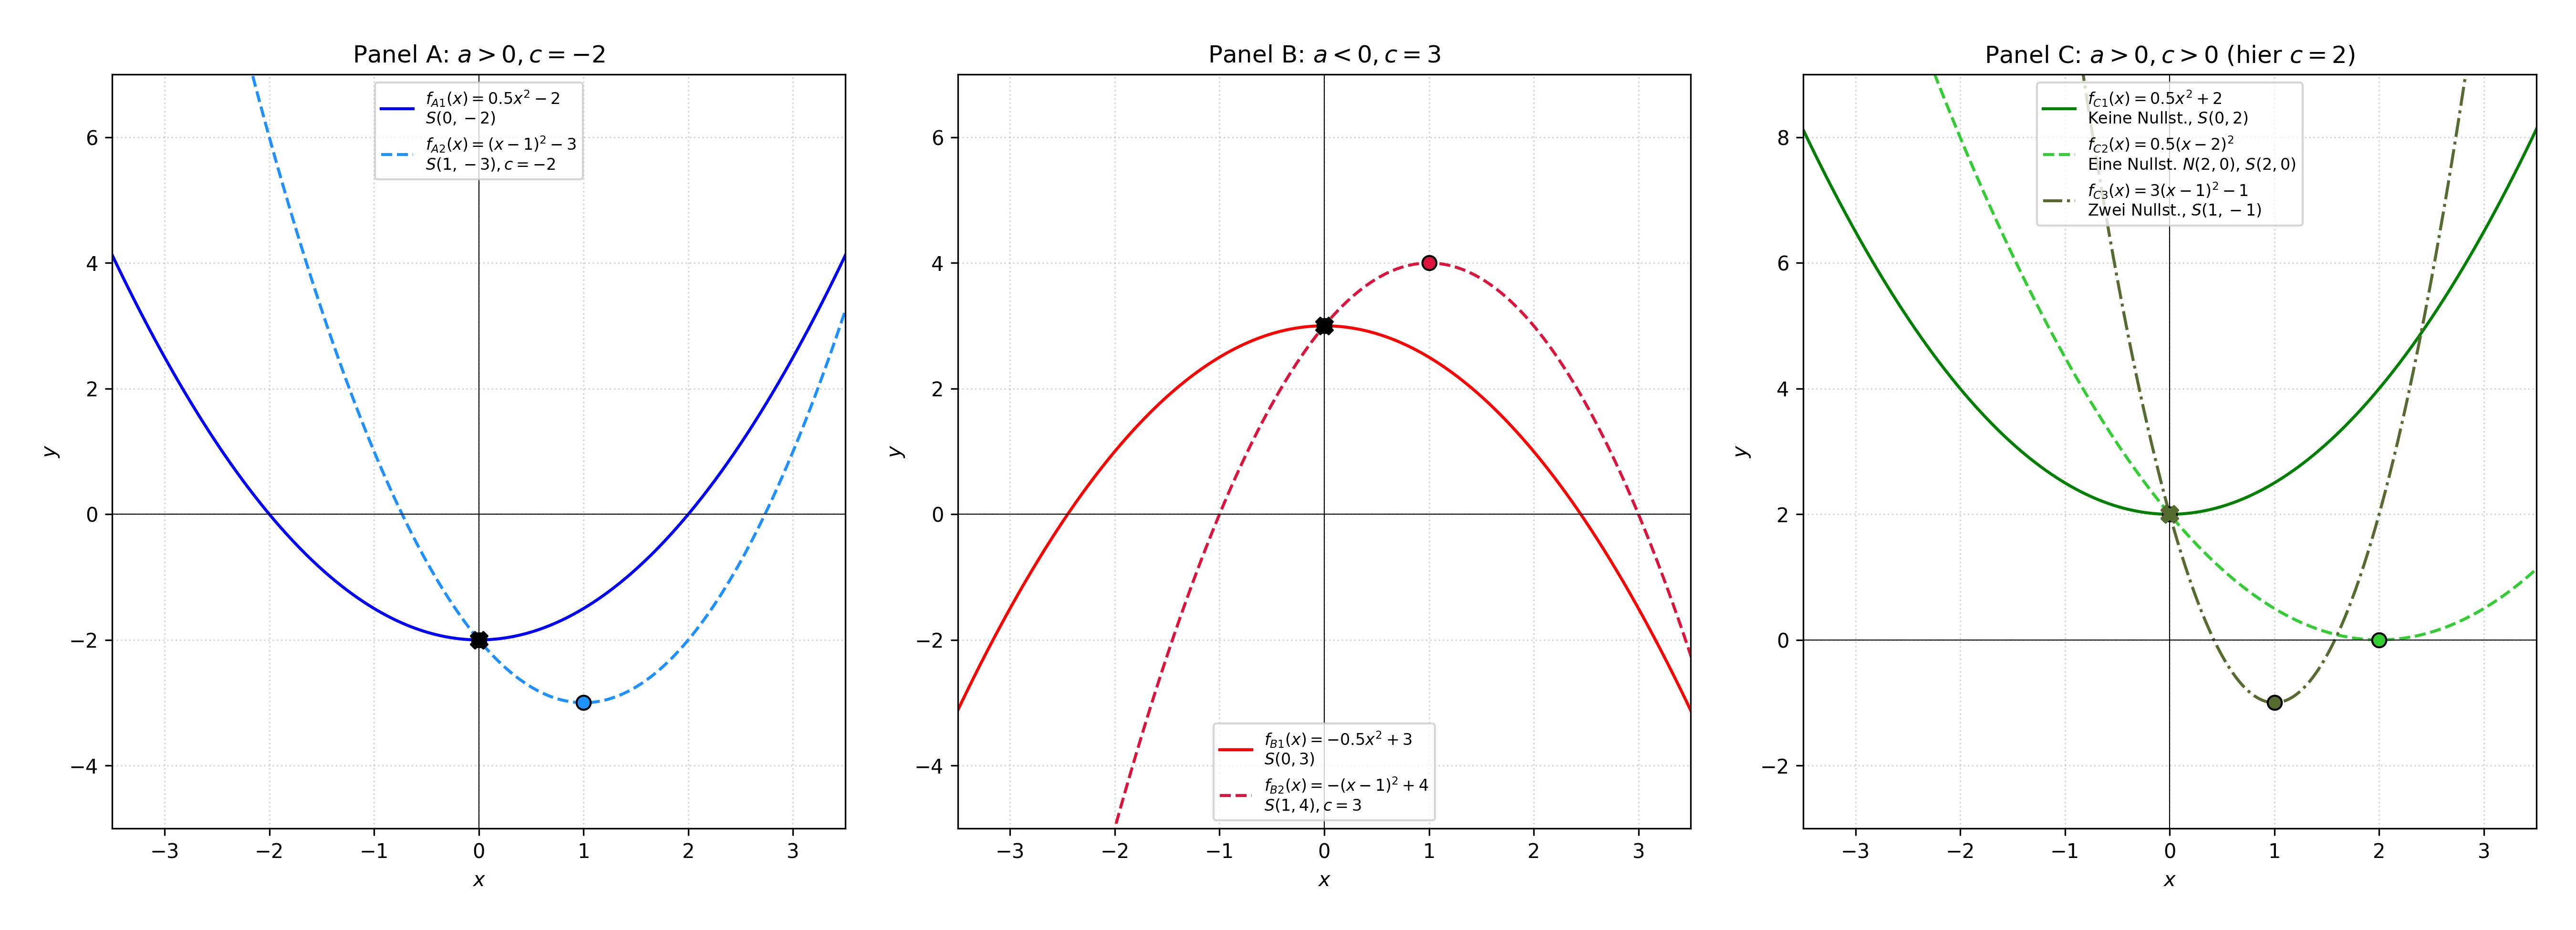
\includegraphics[width=0.9\textwidth]{grafiken/parabeln_teil2_szenarien_ac.png}
    % --- Beschreibung der zusammengefassten Skizze für Teil 2 ---
    % Die Abbildung ist in drei Panels (A, B, C) unterteilt oder stellt die Szenarien klar getrennt dar.
    % Panel A (für 2a): a > 0, c = -2. Zeigt zwei mögliche nach oben geöffnete Parabeln, die die y-Achse bei -2 schneiden und jeweils zwei Nullstellen haben. Eine mit S(0|-2), eine mit S z.B. S(1|-3).
    % Panel B (für 2b): a < 0, c = 3. Zeigt zwei mögliche nach unten geöffnete Parabeln, die die y-Achse bei 3 schneiden und jeweils zwei Nullstellen haben. Eine mit S(0|3), eine mit S z.B. S(1|4).
    % Panel C (für 2c): a > 0, c > 0 (z.B. c=4). Zeigt DREI mögliche nach oben geöffnete Parabeln, die die y-Achse bei c>0 schneiden:
    %    C1: Keine Nullstellen (Scheitelpunkt y_S > 0).
    %    C2: Eine Nullstelle (Scheitelpunkt y_S = 0, berührt x-Achse).
    %    C3: Zwei Nullstellen (Scheitelpunkt y_S < 0).
    % Alle Parabeln sind entsprechend ihrer Parameter (Öffnung, y-Achsenabschnitt) gezeichnet.
    \captionof{figure}{Skizzensammlung für Teil 2: Szenarien basierend auf Öffnungsfaktor $a$ und y-Achsenabschnitt $c$.}
    \label{fig:parabeln_teil2_szenarien_ac}
    \end{center}

\end{enumerate}

\end{loesungsumgebung}


\begin{aufgabenumgebung}{Grenzwerte im Unendlichen}
Bestimme das Verhalten der folgenden Polynomfunktionen für $x \to \infty$ und $x \to -\infty$:
\begin{enumerate}
    \item $f(x) = -x^5 + 3x^2 - 7$
    \item $g(x) = 0.1x^6 - 1000x + 200$
    \item $h(x) = (2-x)(x+1)(x-3)$ (Tipp: Multipliziere die Klammern nicht vollständig aus. Überlege dir, was der Term mit der höchsten Potenz sein wird und welches Vorzeichen sein Koeffizient hat.)
\end{enumerate}
\end{aufgabenumgebung}

\begin{loesungsumgebung}[loes:grenzwerte-unendlich]{Grenzwerte im Unendlichen}
Das Verhalten einer Polynomfunktion für $x \to \pm\infty$ wird durch den Term mit der höchsten Potenz von $x$ (dem Leitterm) bestimmt.

\begin{enumerate}[label=(\alph*)]
    \item \textbf{Funktion $f(x) = -x^5 + 3x^2 - 7$} \\
    Der Leitterm ist $-x^5$.
    \begin{itemize}
        \item Für $x \to \infty$: \\
        $x^5 \to \infty$. Somit $-x^5 \to -\infty$.
        Also gilt: $\lim_{x \to \infty} f(x) = -\infty$.
        \item Für $x \to -\infty$: \\
        $x^5 \to -\infty$ (da der Exponent 5 ungerade ist). Somit $-x^5 \to -(-\infty) = \infty$.
        Also gilt: $\lim_{x \to -\infty} f(x) = \infty$.
    \end{itemize}

    \item \textbf{Funktion $g(x) = 0.1x^6 - 1000x + 200$} \\
    Der Leitterm ist $0.1x^6$. Der Koeffizient $0.1$ ist positiv.
    \begin{itemize}
        \item Für $x \to \infty$: \\
        $x^6 \to \infty$. Da $0.1 > 0$, ist $0.1x^6 \to \infty$.
        Also gilt: $\lim_{x \to \infty} g(x) = \infty$.
        \item Für $x \to -\infty$: \\
        $x^6 \to \infty$ (da der Exponent 6 gerade ist). Da $0.1 > 0$, ist $0.1x^6 \to \infty$.
        Also gilt: $\lim_{x \to -\infty} g(x) = \infty$.
    \end{itemize}

    \item \textbf{Funktion $h(x) = (2-x)(x+1)(x-3)$} \\
    Um den Leitterm zu bestimmen, ohne vollständig auszumultiplizieren, betrachten wir die Terme mit der höchsten Potenz von $x$ in jeder Klammer: $(-x)$, $(x)$ und $(x)$.
    Das Produkt dieser Terme ist $(-x) \cdot (x) \cdot (x) = -x^3$.
    Der Leitterm ist also $-x^3$.
    \begin{itemize}
        \item Für $x \to \infty$: \\
        $x^3 \to \infty$. Somit $-x^3 \to -\infty$.
        Also gilt: $\lim_{x \to \infty} h(x) = -\infty$.
        \item Für $x \to -\infty$: \\
        $x^3 \to -\infty$ (da der Exponent 3 ungerade ist). Somit $-x^3 \to -(-\infty) = \infty$.
        Also gilt: $\lim_{x \to -\infty} h(x) = \infty$.
    \end{itemize}
\end{enumerate}

\begin{merksatzumgebung}{Globalverhalten von Polynomen}
Das Verhalten eines Polynoms $P(x) = a_n x^n + a_{n-1}x^{n-1} + \dots + a_1 x + a_0$ für $x \to \pm\infty$ hängt nur vom Leitterm $a_n x^n$ ab:
\begin{itemize}
    \item Ist $n$ \textbf{gerade}:
    \begin{itemize}
        \item Wenn $a_n > 0$: $P(x) \to \infty$ für $x \to \infty$ und $P(x) \to \infty$ für $x \to -\infty$ (kommt von links oben, geht nach rechts oben).
        \item Wenn $a_n < 0$: $P(x) \to -\infty$ für $x \to \infty$ und $P(x) \to -\infty$ für $x \to -\infty$ (kommt von links unten, geht nach rechts unten).
    \end{itemize}
    \item Ist $n$ \textbf{ungerade}:
    \begin{itemize}
        \item Wenn $a_n > 0$: $P(x) \to \infty$ für $x \to \infty$ und $P(x) \to -\infty$ für $x \to -\infty$ (kommt von links unten, geht nach rechts oben).
        \item Wenn $a_n < 0$: $P(x) \to -\infty$ für $x \to \infty$ und $P(x) \to \infty$ für $x \to -\infty$ (kommt von links oben, geht nach rechts unten).
    \end{itemize}
\end{itemize}
\end{merksatzumgebung}

\end{loesungsumgebung}

\begin{aufgabenumgebung}{Polynom 3. Grades: Wertetabelle, Graph und Verhalten}
Betrachten wir die Polynomfunktion 3. Grades:
\[ f(x) = x^3 - 3x^2 + 4 \]
\begin{enumerate}[label=(\alph*)]
    \item \textbf{Wertetabelle erstellen:} Erstelle eine Wertetabelle für $f(x)$ für die ganzzahligen $x$-Werte von $-2$ bis $3$.
    \begin{center}
    \begin{tabular}{c||c|c|c|c|c|c}
    $x$ & -2 & -1 & 0 & 1 & 2 & 3 \\
    \hline
    $f(x)$ &    &    &   &   &   &   \\
    \end{tabular}
    \end{center}
    \item \textbf{Graph skizzieren:} Zeichne den Graphen der Funktion $f(x)$ in ein Koordinatensystem, indem du die Punkte aus deiner Wertetabelle verbindest. Wähle die Achsenskalierung so, dass alle berechneten Punkte gut sichtbar sind.
    \item \textbf{Besondere Punkte identifizieren:}
    \begin{itemize}
        \item Kannst du anhand deiner Wertetabelle und/oder deiner Skizze vermutliche \textbf{Nullstellen} der Funktion erkennen? Notiere die $x$-Werte.
        \item Fallen dir in deiner Skizze Bereiche auf, die lokale \textbf{Hochpunkte} (Berggipfel) oder \textbf{Tiefpunkte} (Talsohlen) sein könnten? Markiere diese im Graphen und notiere die ungefähren Koordinaten $(x|y)$ dieser Punkte, soweit du sie aus deiner Tabelle oder Zeichnung ablesen kannst.
    \end{itemize}
    \item \textbf{Verhalten im Unendlichen (Globalverhalten):}
    Du kennst bereits das Konzept des Grenzwerts (Limes). Überlege dir, wie sich die Funktion $f(x) = x^3 - 3x^2 + 4$ für sehr große positive und sehr große negative $x$-Werte verhält. Welcher Term in der Funktionsgleichung dominiert das Verhalten für $x \to \infty$ und $x \to -\infty$?
    \begin{itemize}
        \item Was erwartest du für $f(x)$, wenn $x \to \infty$ (d.h. $x$ wird beliebig groß positiv)?
        \item Was erwartest du für $f(x)$, wenn $x \to -\infty$ (d.h. $x$ wird beliebig groß negativ)?
    \end{itemize}
    Passt dieses Verhalten zu deiner Skizze?
\end{enumerate}
\end{aufgabenumgebung}


\begin{loesungsumgebung}[loes:polynom-3-grad-analyse]{Polynom 3. Grades: Wertetabelle, Graph und Verhalten}
Wir untersuchen die Polynomfunktion $f(x) = x^3 - 3x^2 + 4$.

\begin{enumerate}[label=(\alph*)]
    \item \textbf{Wertetabelle erstellen:}
    Wir berechnen die Funktionswerte $f(x)$ für die ganzzahligen $x$-Werte von $-2$ bis $3$:
    \begin{itemize}
        \item $f(-2) = (-2)^3 - 3(-2)^2 + 4 = -8 - 3(4) + 4 = -8 - 12 + 4 = -16$
        \item $f(-1) = (-1)^3 - 3(-1)^2 + 4 = -1 - 3(1) + 4 = -1 - 3 + 4 = 0$
        \item $f(0) = (0)^3 - 3(0)^2 + 4 = 0 - 0 + 4 = 4$
        \item $f(1) = (1)^3 - 3(1)^2 + 4 = 1 - 3(1) + 4 = 1 - 3 + 4 = 2$
        \item $f(2) = (2)^3 - 3(2)^2 + 4 = 8 - 3(4) + 4 = 8 - 12 + 4 = 0$
        \item $f(3) = (3)^3 - 3(3)^2 + 4 = 27 - 3(9) + 4 = 27 - 27 + 4 = 4$
    \end{itemize}
    Die ausgefüllte Wertetabelle sieht wie folgt aus:
    \begin{center}
    \begin{tabular}{c||c|c|c|c|c|c}
    $x$ & -2 & -1 & 0 & 1 & 2 & 3 \\
    \hline
    $f(x)$ & -16 & 0 & 4 & 2 & 0 & 4 \\
    \end{tabular}
    \end{center}

    \item \textbf{Graph skizzieren:}
    Der Graph wird gezeichnet, indem die Punkte $(-2|-16)$, $(-1|0)$, $(0|4)$, $(1|2)$, $(2|0)$ und $(3|4)$ in ein Koordinatensystem eingetragen und sinnvoll verbunden werden.
    \begin{center}
    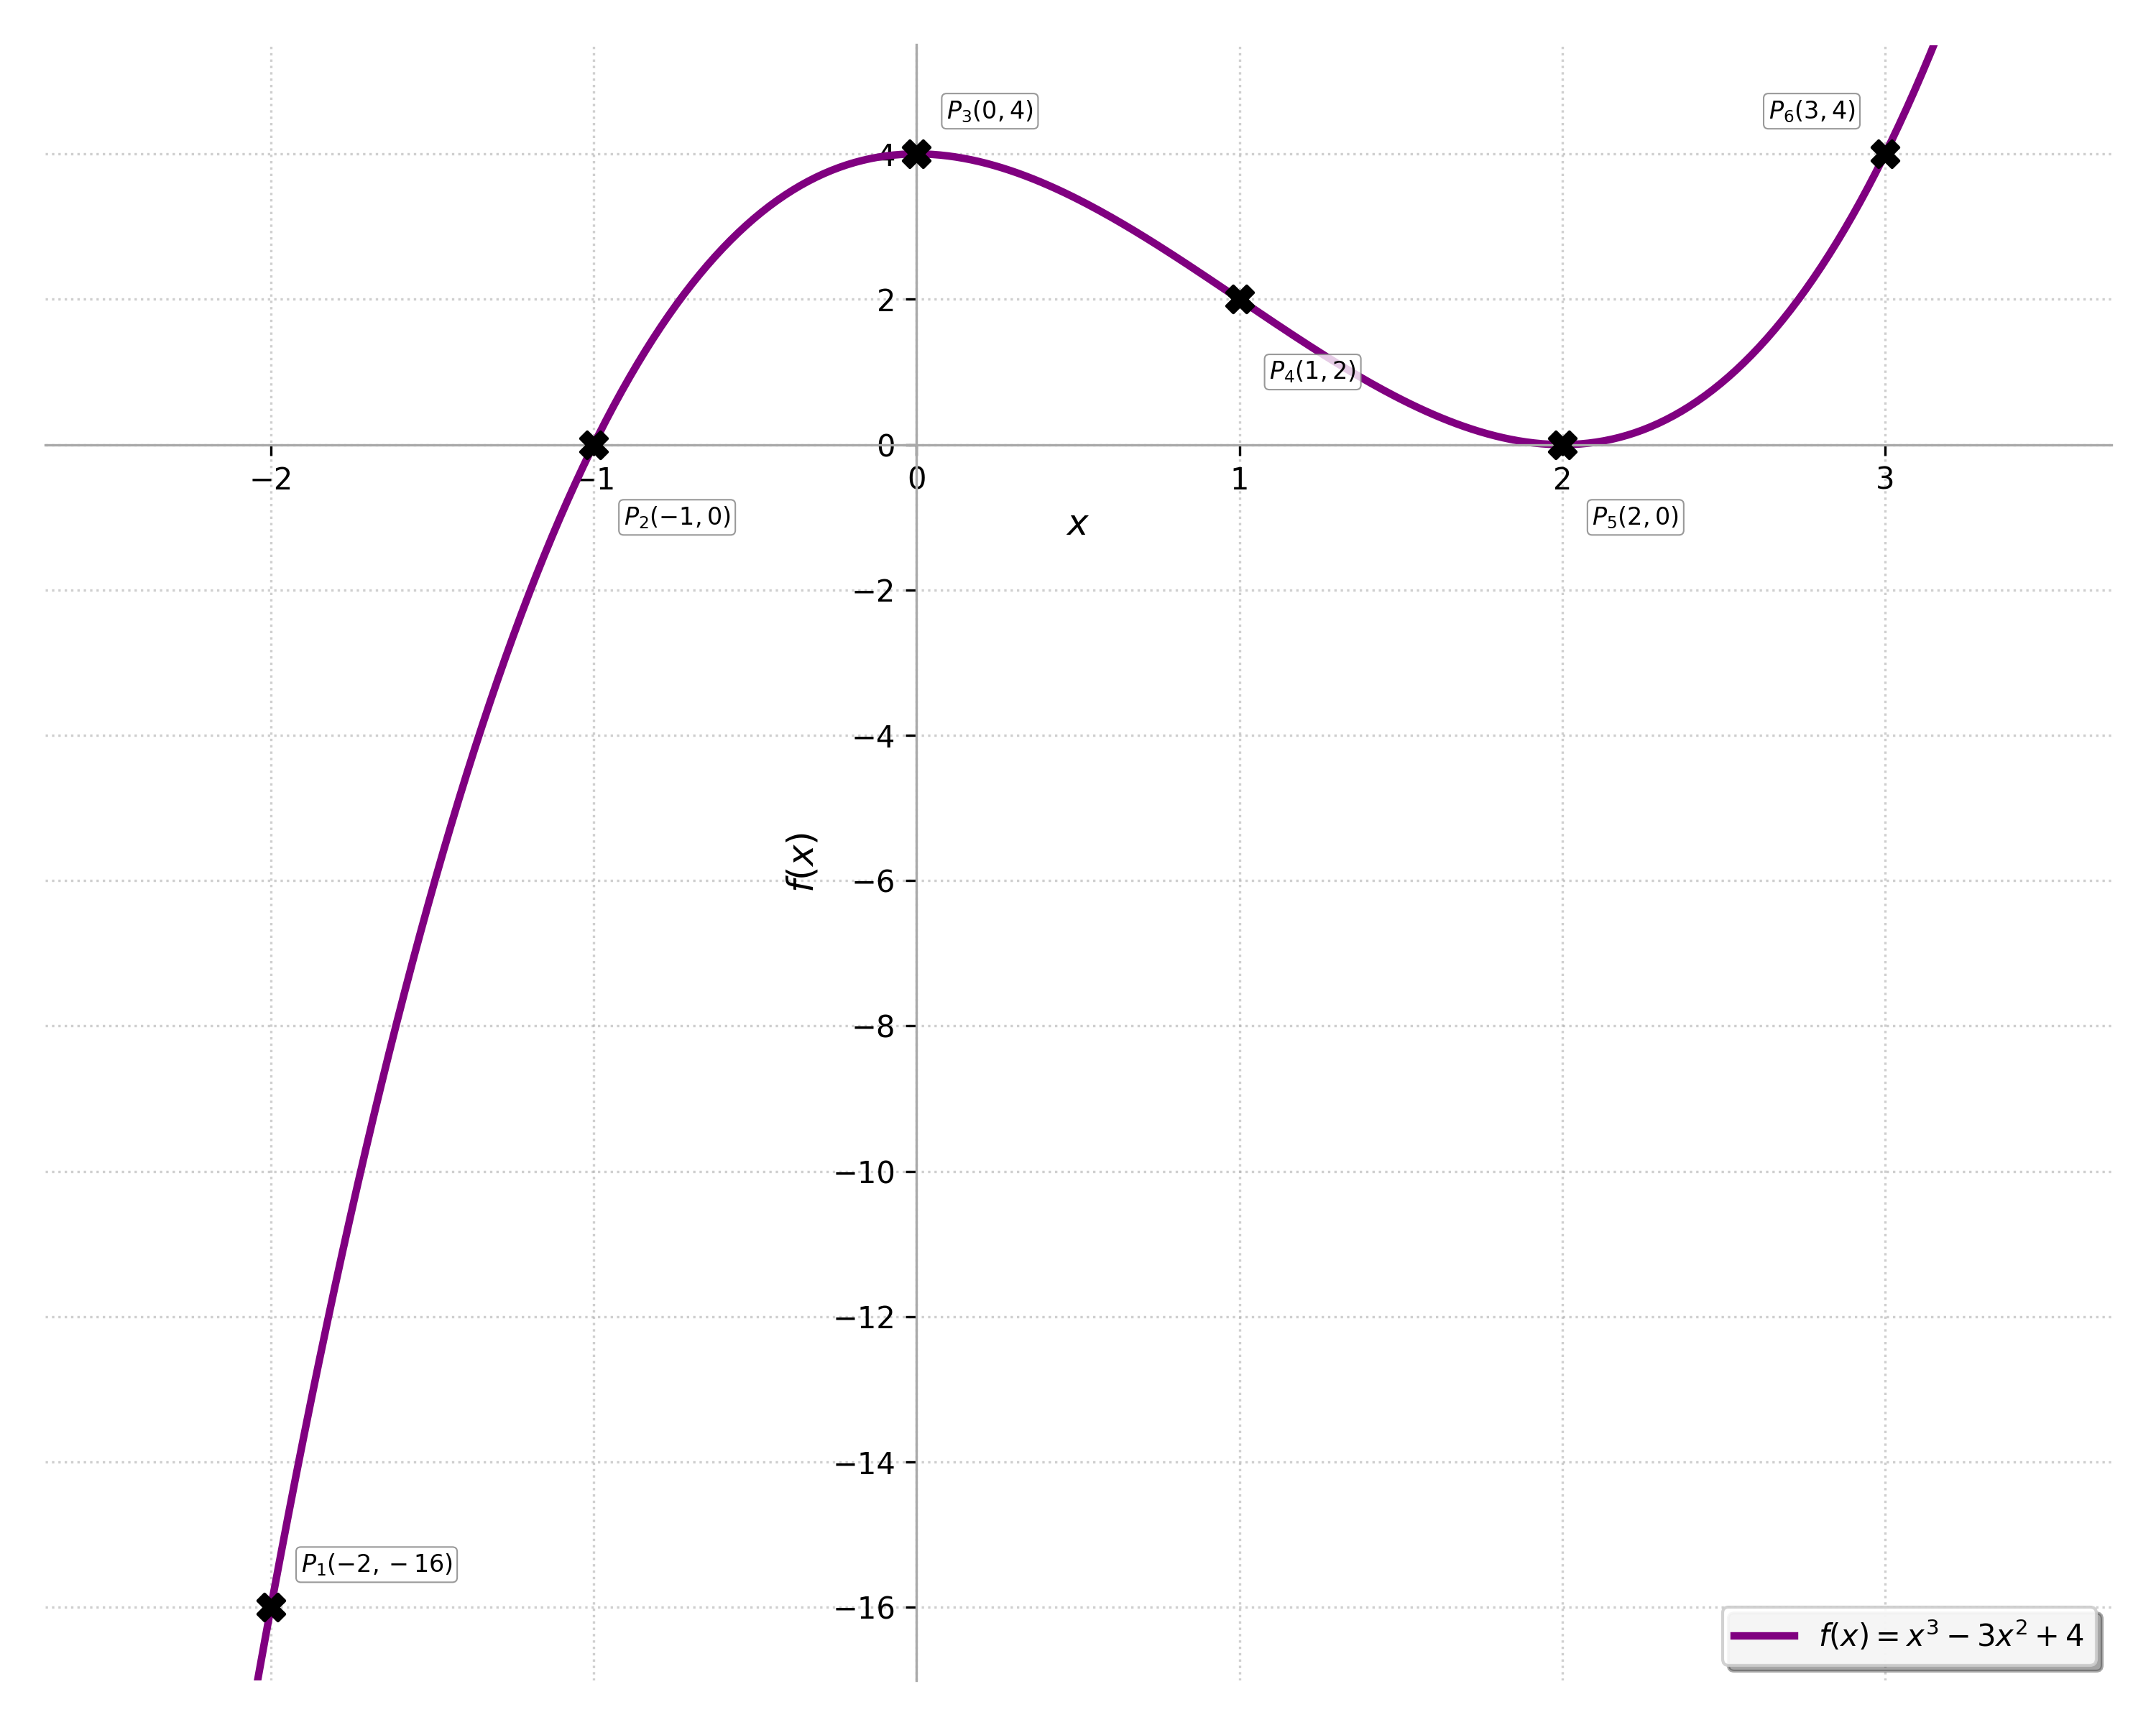
\includegraphics[width=0.8\textwidth]{grafiken/polynom_f_graph.png}
    % --- Beschreibung der Grafik ---
    % Die Grafik zeigt ein kartesisches Koordinatensystem.
    % Die x-Achse ist beschriftet und skaliert, um den Bereich von ca. -2.5 bis 3.5 abzudecken.
    % Die y-Achse ist beschriftet und skaliert, um den Bereich von ca. -17 bis 5 abzudecken.
    % Der Graph der Funktion f(x) = x^3 - 3x^2 + 4 ist als glatte Kurve durch die berechneten Punkte gezeichnet.
    % Die Punkte (-2|-16), (-1|0), (0|4), (1|2), (2|0), (3|4) sind auf der Kurve erkennbar.
    % Die Kurve zeigt einen Anstieg bis zu einem lokalen Maximum, fällt dann zu einem lokalen Minimum und steigt danach wieder an.
    \captionof{figure}{Skizze des Graphen der Funktion $f(x) = x^3 - 3x^2 + 4$ basierend auf der Wertetabelle.}
    \label{fig:polynom_f_graph}
    \end{center}

    \item \textbf{Besondere Punkte identifizieren:}
    \begin{itemize}
        \item \textbf{Vermutliche Nullstellen:}
        Anhand der Wertetabelle sehen wir, dass $f(-1)=0$ und $f(2)=0$. Daher sind $x_1 = -1$ und $x_2 = 2$ vermutliche Nullstellen der Funktion. Die Skizze bestätigt, dass der Graph an diesen Stellen die x-Achse schneidet bzw. berührt.
        \item \textbf{Lokale Hochpunkte und Tiefpunkte:}
        Betrachtet man die Wertetabelle und die Skizze:
        \begin{itemize}
            \item Zwischen $x=-1$ ($f(-1)=0$) und $x=1$ ($f(1)=2$) steigt der Graph bis zu $f(0)=4$ an und fällt dann wieder. Daher liegt ein vermutlicher \textbf{lokaler Hochpunkt (Berggipfel)} bei oder nahe $(0|4)$.
            \item Zwischen $x=1$ ($f(1)=2$) und $x=3$ ($f(3)=4$) fällt der Graph bis zu $f(2)=0$ und steigt dann wieder an. Daher liegt ein vermutlicher \textbf{lokaler Tiefpunkt (Talsohle)} bei oder nahe $(2|0)$. Die Tatsache, dass $x=2$ auch eine Nullstelle ist, deutet darauf hin, dass der Graph die x-Achse hier berührt.
        \end{itemize}
        Die ungefähren Koordinaten sind: Lokaler Hochpunkt $\approx (0|4)$ und lokaler Tiefpunkt $\approx (2|0)$.
    \end{itemize}

    \item \textbf{Verhalten im Unendlichen (Globalverhalten):}
    Die Funktion ist $f(x) = x^3 - 3x^2 + 4$. Der Term, der das Verhalten für $x \to \pm\infty$ dominiert, ist der Term mit der höchsten Potenz von $x$, also $x^3$.
    \begin{itemize}
        \item \textbf{Was erwartest du für $f(x)$, wenn $x \to \infty$?} \\
        Wenn $x$ sehr groß positiv wird ($x \to \infty$), wird $x^3$ ebenfalls sehr groß positiv ($x^3 \to \infty$).
        Daher erwarten wir $\lim_{x \to \infty} f(x) = \infty$.
        \item \textbf{Was erwartest du für $f(x)$, wenn $x \to -\infty$?} \\
        Wenn $x$ sehr groß negativ wird ($x \to -\infty$), wird $x^3$ ebenfalls sehr groß negativ ($x^3 \to -\infty$, da der Exponent ungerade ist).
        Daher erwarten wir $\lim_{x \to -\infty} f(x) = -\infty$.
    \end{itemize}
    \textbf{Passt dieses Verhalten zu deiner Skizze?} \\
    Ja, dieses Verhalten passt zur Skizze. Die Skizze deutet an, dass der Graph von links unten kommt ($x \to -\infty, f(x) \to -\infty$), dann ansteigt, lokale Extrema bildet und schließlich nach rechts oben weiter verläuft ($x \to \infty, f(x) \to \infty$).
\end{enumerate}

\end{loesungsumgebung}